% Options for packages loaded elsewhere
\PassOptionsToPackage{unicode}{hyperref}
\PassOptionsToPackage{hyphens}{url}
\PassOptionsToPackage{dvipsnames,svgnames,x11names}{xcolor}
%
\documentclass[
  letterpaper,
  DIV=11,
  numbers=noendperiod]{scrartcl}

\usepackage{amsmath,amssymb}
\usepackage{iftex}
\ifPDFTeX
  \usepackage[T1]{fontenc}
  \usepackage[utf8]{inputenc}
  \usepackage{textcomp} % provide euro and other symbols
\else % if luatex or xetex
  \usepackage{unicode-math}
  \defaultfontfeatures{Scale=MatchLowercase}
  \defaultfontfeatures[\rmfamily]{Ligatures=TeX,Scale=1}
\fi
\usepackage{lmodern}
\ifPDFTeX\else  
    % xetex/luatex font selection
\fi
% Use upquote if available, for straight quotes in verbatim environments
\IfFileExists{upquote.sty}{\usepackage{upquote}}{}
\IfFileExists{microtype.sty}{% use microtype if available
  \usepackage[]{microtype}
  \UseMicrotypeSet[protrusion]{basicmath} % disable protrusion for tt fonts
}{}
\makeatletter
\@ifundefined{KOMAClassName}{% if non-KOMA class
  \IfFileExists{parskip.sty}{%
    \usepackage{parskip}
  }{% else
    \setlength{\parindent}{0pt}
    \setlength{\parskip}{6pt plus 2pt minus 1pt}}
}{% if KOMA class
  \KOMAoptions{parskip=half}}
\makeatother
\usepackage{xcolor}
\setlength{\emergencystretch}{3em} % prevent overfull lines
\setcounter{secnumdepth}{-\maxdimen} % remove section numbering
% Make \paragraph and \subparagraph free-standing
\makeatletter
\ifx\paragraph\undefined\else
  \let\oldparagraph\paragraph
  \renewcommand{\paragraph}{
    \@ifstar
      \xxxParagraphStar
      \xxxParagraphNoStar
  }
  \newcommand{\xxxParagraphStar}[1]{\oldparagraph*{#1}\mbox{}}
  \newcommand{\xxxParagraphNoStar}[1]{\oldparagraph{#1}\mbox{}}
\fi
\ifx\subparagraph\undefined\else
  \let\oldsubparagraph\subparagraph
  \renewcommand{\subparagraph}{
    \@ifstar
      \xxxSubParagraphStar
      \xxxSubParagraphNoStar
  }
  \newcommand{\xxxSubParagraphStar}[1]{\oldsubparagraph*{#1}\mbox{}}
  \newcommand{\xxxSubParagraphNoStar}[1]{\oldsubparagraph{#1}\mbox{}}
\fi
\makeatother

\usepackage{color}
\usepackage{fancyvrb}
\newcommand{\VerbBar}{|}
\newcommand{\VERB}{\Verb[commandchars=\\\{\}]}
\DefineVerbatimEnvironment{Highlighting}{Verbatim}{commandchars=\\\{\}}
% Add ',fontsize=\small' for more characters per line
\usepackage{framed}
\definecolor{shadecolor}{RGB}{241,243,245}
\newenvironment{Shaded}{\begin{snugshade}}{\end{snugshade}}
\newcommand{\AlertTok}[1]{\textcolor[rgb]{0.68,0.00,0.00}{#1}}
\newcommand{\AnnotationTok}[1]{\textcolor[rgb]{0.37,0.37,0.37}{#1}}
\newcommand{\AttributeTok}[1]{\textcolor[rgb]{0.40,0.45,0.13}{#1}}
\newcommand{\BaseNTok}[1]{\textcolor[rgb]{0.68,0.00,0.00}{#1}}
\newcommand{\BuiltInTok}[1]{\textcolor[rgb]{0.00,0.23,0.31}{#1}}
\newcommand{\CharTok}[1]{\textcolor[rgb]{0.13,0.47,0.30}{#1}}
\newcommand{\CommentTok}[1]{\textcolor[rgb]{0.37,0.37,0.37}{#1}}
\newcommand{\CommentVarTok}[1]{\textcolor[rgb]{0.37,0.37,0.37}{\textit{#1}}}
\newcommand{\ConstantTok}[1]{\textcolor[rgb]{0.56,0.35,0.01}{#1}}
\newcommand{\ControlFlowTok}[1]{\textcolor[rgb]{0.00,0.23,0.31}{\textbf{#1}}}
\newcommand{\DataTypeTok}[1]{\textcolor[rgb]{0.68,0.00,0.00}{#1}}
\newcommand{\DecValTok}[1]{\textcolor[rgb]{0.68,0.00,0.00}{#1}}
\newcommand{\DocumentationTok}[1]{\textcolor[rgb]{0.37,0.37,0.37}{\textit{#1}}}
\newcommand{\ErrorTok}[1]{\textcolor[rgb]{0.68,0.00,0.00}{#1}}
\newcommand{\ExtensionTok}[1]{\textcolor[rgb]{0.00,0.23,0.31}{#1}}
\newcommand{\FloatTok}[1]{\textcolor[rgb]{0.68,0.00,0.00}{#1}}
\newcommand{\FunctionTok}[1]{\textcolor[rgb]{0.28,0.35,0.67}{#1}}
\newcommand{\ImportTok}[1]{\textcolor[rgb]{0.00,0.46,0.62}{#1}}
\newcommand{\InformationTok}[1]{\textcolor[rgb]{0.37,0.37,0.37}{#1}}
\newcommand{\KeywordTok}[1]{\textcolor[rgb]{0.00,0.23,0.31}{\textbf{#1}}}
\newcommand{\NormalTok}[1]{\textcolor[rgb]{0.00,0.23,0.31}{#1}}
\newcommand{\OperatorTok}[1]{\textcolor[rgb]{0.37,0.37,0.37}{#1}}
\newcommand{\OtherTok}[1]{\textcolor[rgb]{0.00,0.23,0.31}{#1}}
\newcommand{\PreprocessorTok}[1]{\textcolor[rgb]{0.68,0.00,0.00}{#1}}
\newcommand{\RegionMarkerTok}[1]{\textcolor[rgb]{0.00,0.23,0.31}{#1}}
\newcommand{\SpecialCharTok}[1]{\textcolor[rgb]{0.37,0.37,0.37}{#1}}
\newcommand{\SpecialStringTok}[1]{\textcolor[rgb]{0.13,0.47,0.30}{#1}}
\newcommand{\StringTok}[1]{\textcolor[rgb]{0.13,0.47,0.30}{#1}}
\newcommand{\VariableTok}[1]{\textcolor[rgb]{0.07,0.07,0.07}{#1}}
\newcommand{\VerbatimStringTok}[1]{\textcolor[rgb]{0.13,0.47,0.30}{#1}}
\newcommand{\WarningTok}[1]{\textcolor[rgb]{0.37,0.37,0.37}{\textit{#1}}}

\providecommand{\tightlist}{%
  \setlength{\itemsep}{0pt}\setlength{\parskip}{0pt}}\usepackage{longtable,booktabs,array}
\usepackage{calc} % for calculating minipage widths
% Correct order of tables after \paragraph or \subparagraph
\usepackage{etoolbox}
\makeatletter
\patchcmd\longtable{\par}{\if@noskipsec\mbox{}\fi\par}{}{}
\makeatother
% Allow footnotes in longtable head/foot
\IfFileExists{footnotehyper.sty}{\usepackage{footnotehyper}}{\usepackage{footnote}}
\makesavenoteenv{longtable}
\usepackage{graphicx}
\makeatletter
\def\maxwidth{\ifdim\Gin@nat@width>\linewidth\linewidth\else\Gin@nat@width\fi}
\def\maxheight{\ifdim\Gin@nat@height>\textheight\textheight\else\Gin@nat@height\fi}
\makeatother
% Scale images if necessary, so that they will not overflow the page
% margins by default, and it is still possible to overwrite the defaults
% using explicit options in \includegraphics[width, height, ...]{}
\setkeys{Gin}{width=\maxwidth,height=\maxheight,keepaspectratio}
% Set default figure placement to htbp
\makeatletter
\def\fps@figure{htbp}
\makeatother

\KOMAoption{captions}{tableheading}
\makeatletter
\@ifpackageloaded{caption}{}{\usepackage{caption}}
\AtBeginDocument{%
\ifdefined\contentsname
  \renewcommand*\contentsname{Table of contents}
\else
  \newcommand\contentsname{Table of contents}
\fi
\ifdefined\listfigurename
  \renewcommand*\listfigurename{List of Figures}
\else
  \newcommand\listfigurename{List of Figures}
\fi
\ifdefined\listtablename
  \renewcommand*\listtablename{List of Tables}
\else
  \newcommand\listtablename{List of Tables}
\fi
\ifdefined\figurename
  \renewcommand*\figurename{Figure}
\else
  \newcommand\figurename{Figure}
\fi
\ifdefined\tablename
  \renewcommand*\tablename{Table}
\else
  \newcommand\tablename{Table}
\fi
}
\@ifpackageloaded{float}{}{\usepackage{float}}
\floatstyle{ruled}
\@ifundefined{c@chapter}{\newfloat{codelisting}{h}{lop}}{\newfloat{codelisting}{h}{lop}[chapter]}
\floatname{codelisting}{Listing}
\newcommand*\listoflistings{\listof{codelisting}{List of Listings}}
\makeatother
\makeatletter
\makeatother
\makeatletter
\@ifpackageloaded{caption}{}{\usepackage{caption}}
\@ifpackageloaded{subcaption}{}{\usepackage{subcaption}}
\makeatother

\ifLuaTeX
  \usepackage{selnolig}  % disable illegal ligatures
\fi
\usepackage{bookmark}

\IfFileExists{xurl.sty}{\usepackage{xurl}}{} % add URL line breaks if available
\urlstyle{same} % disable monospaced font for URLs
\hypersetup{
  pdftitle={Paper},
  pdfauthor={Hao Zhu},
  colorlinks=true,
  linkcolor={blue},
  filecolor={Maroon},
  citecolor={Blue},
  urlcolor={Blue},
  pdfcreator={LaTeX via pandoc}}


\title{Paper}
\author{Hao Zhu}
\date{2025-03-15}

\begin{document}
\maketitle


(Title)

\section{Introduction}\label{introduction}

Human learning hinges on the ability to recognize and interpret
predictive cues in the environment. Classic work in associative learning
has shown that when two or more cues consistently appear together, their
interactions can be competitive---where a dominant cue ``blocks''
another from acquiring associative strength---or facilitative, in which
cues mutually boost each other's predictive value. These phenomena play
a fundamental role not only in understanding how people learn
cause-effect relationships but also in broader psychological processes
such as selective attention, cognitive inference, and clinical outcomes
related to anxiety and stress. In the dissertation by Alhazmi (2022), a
series of experiments explored the interplay between these different
styles of cue interaction---particularly examining why some individuals
tend toward facilitative (or ``noncompetitive'') learning while others
exhibit more canonical patterns of cue competition. The present paper
focuses on Experiment 4 of that work, in which I conducted a detailed
data analysis to investigate individual differences in cue interaction
style (competitive vs.~facilitative) and whether their styles are
related to anxiety, depression, and stress measures, and how reversal
learning might influence these interactions.

This introductory section provides an overview of the theoretical basis
for cue interaction, including both classical associative models and
more contemporary accounts that incorporate higher-order cognitive
processes.

Theoretical accounts of cue interaction have historically emphasized how
cues compete for associative strength, a process often referred to as
``cue competition.'' Early associative models (e.g., Bush \& Mosteller,
1951, 1955) proposed that the predictive value of any given cue depends
solely on its individual correlation with the outcome. This view was
challenged by the influential Rescorla-Wagner model (Rescorla \& Wagner,
1972), which introduced the concept of a summed prediction error.
According to this model, cues presented in compound share a limited pool
of associative strength; a cue that is already a strong predictor of an
outcome will ``block'' new cues from acquiring substantial associative
strength (Kamin, 1968; Rescorla \& Wagner, 1972). Later theories,
particularly attentional models (Mackintosh, 1975; Pearce \& Hall,
1980), posited that competition stems not just from summed prediction
errors but also from changes in the amount of attention allocated to
each cue.

However, accumulating evidence suggests that cues can also facilitate
one another---rather than compete---under certain circumstances (Bouton
et al., 1987; Durlach \& Rescorla, 1980). Such ``cue facilitation''
occurs when the presence of a well-established cue enhances the
predictive value of a novel cue (Batsell Jr \& Batson, 1999). Models
addressing both competition and facilitation often incorporate
within-compound associations---that is, direct links formed between cues
presented together. In the Sometimes-Competing Retrieval (SOCR) model
(Stout \& Miller, 2007), these within-compound associations may either
suppress or augment responding, depending on a ``switching operator''
that governs whether indirect cue activation will interfere with or
bolster responding. Similarly, Pineño's (2007) extension of the
Rescorla-Wagner model assumes that a cue's novelty moderates how
strongly it draws on within-compound associations for its
response---leading sometimes to competition, sometimes to facilitation.
These dual-process models thus capture both the classic competitive
phenomena and the growing body of evidence for cooperative, or
facilitative, interactions among cues.

In addition to these associative mechanisms, propositional and
higher-order reasoning can also influence cue interactions. According to
propositional accounts, human learners form cognitive inferences about
causal relationships, rather than simply accumulating associative
strength through trial-by-trial error signals (Mitchell et al., 2009).
Thus, learners may explicitly reason that ``if Cue A by itself predicts
the outcome, and Cue A together with Cue X produces no change in the
outcome, then Cue X is not causally relevant,'' leading to blocking-like
effects (Cheng \& Novick, 1990; De Houwer \& Beckers, 2003).
Higher-order cognition may similarly generate facilitative effects if
learners reason that a known predictor could boost the effectiveness of
other cues present in the same compound. These propositional processes
need not replace traditional associative mechanisms; indeed, both
conscious inference and lower-level associative learning may jointly
shape how cues compete or facilitate one another under varying task
conditions (Mitchell et al., 2009).

Another theoretical perspective on cue interaction revolves around
\textbf{within-compound associations}, which are direct links formed
between cues that are presented simultaneously. Rather than focusing
exclusively on how each cue associates with an outcome, this view
emphasizes that cues can become associated with each other---sometimes
resulting in one cue retrieving the memory of its partner, which in turn
activates the representation of the shared outcome (Melchers et al.,
2004; Miller \& Matzel, 1988). This mechanism can explain why, for
instance, reinforcing one element of a compound (A) in a later stage may
retrospectively weaken or enhance responses to the other (X), even when
X is not explicitly retrained---an effect not easily handled by
standard, purely competitive models. Recent formulations, such as
Pineño's (2007) model or the Sometimes-Competing Retrieval (SOCR) model
(Stout \& Miller, 2007), specifically integrate within-compound
associations to account for both \textbf{competitive} interactions (when
indirect retrieval suppresses responding) and \textbf{facilitative}
interactions (when indirect retrieval augments responding). By focusing
on how cues become interconnected, these approaches help clarify why
certain learners show noncompetitive or ``excessive'' associative
patterns that can, in clinical populations, manifest as overgeneralized
fear or heightened sensitivity to redundant cues.

Taken together, these perspectives underscore how cue interaction can
manifest in both competitive and facilitative patterns, shaped by
propositional reasoning as well as by within-compound associations. In
the fourth experiment of Alhazmi's (2022) dissertation, these themes
converge in a paradigm specifically designed to capture variability in
cue interaction styles under carefully controlled conditions. The next
sections detail how I reanalyzed the dataset from this experiment,
leveraging advanced statistical methods to explore (1) whether
individual shows differences in cue competition or facilitation, (2) how
these differences might correlate with measures of anxiety, depression,
and stress, and (3) how the experimental manipulation of outcome
reversals might influence these interactions.

\textbf{Description of the Fourth Experiment}

Experiment~4 was developed to determine how within-compound associations
might tilt cue interaction toward competitive or facilitative patterns,
and whether these individual tendencies align with varying levels of
anxiety, depression, and stress. The experiment utilized a two-stage
training procedure---initial training followed by compound
trials---culminating in a reversal manipulation that differed between
two groups. What follows is a more detailed account of the procedure:

\textbf{Participants and Design.}

Over 400 adults were recruited online (via Prolific) and randomly
assigned to one of two groups: Control (no outcome reversal) or
Experimental (outcome reversal).

In both groups, each participant was exposed to two cues (A and B)
initially reinforced with coins or bomb outcomes, respectively, so that
A reliably predicted a positive outcome (coins) while B reliably
predicted a negative outcome (bomb).

Stage 1 (Initial Training).

Cues A and B were each presented multiple times (e.g., eight trials per
cue). Consistent with the design, Cue A was always followed by the coin
outcome, while Cue B was always followed by the bomb outcome. This stage
established a baseline expectation that A = coins and B = bomb.

Stage 2 (Compound Training).

Both groups next received extended training over several blocks (e.g.,
seven blocks). These blocks included the original cues (A→coins, B→bomb)
plus newly introduced compound cues:~ AW (A paired with a novel cue W),
75\% resulting in coins and 25\% in bombs.

BZ (B paired with a novel cue Z), 25\% resulting in coins and 75\% in
bombs.

AX (A with novel cue X) and BY (B with novel cue Y), each reinforced
50\% of the time with coins.

These compound trials tested how novel cues (W, X, Y, Z) might
``inherit'' more or less coin or bomb expectancy from their
better-established partners (A or B). Of particular interest were X and
Y, the target cues, since they were paired with opposite outcomes on
half the trials and thus could trend toward coins or bombs depending on
how participants integrated the companion cue's history.

Stage 3 (Reversal Manipulation).

At this point, the Experimental group received a reversal of outcomes
for Cues A and B (i.e., A became bomb, B became coins), while the
Control group continued with the same contingencies (A = coins, B =
bomb).

The logic behind this manipulation was to identify whether people who
relied on strong within-compound associations (especially for cues X or
Y) would update the predictive value of those target cues more
drastically than those who did not depend on within-compound links.

Stage 4 (Final Probe Trials).

Both groups completed additional probe trials in which Cues A, B, X, and
Y were tested individually without explicit feedback, to assess how much
the earlier reversal or continued training influenced each cue's
perceived outcome.

\textbf{Dependent Variables}

\begin{enumerate}
\def\labelenumi{\arabic{enumi}.}
\item
  \textbf{Distance.} A key behavioral measure was how close participants
  positioned themselves (or their avatar) to the anticipated outcome
  location on each trial. By standing near the center when they
  predicted coins (to maximize reward) or retreating toward the edge if
  they expected a bomb (to avoid penalty), participants generated a
  continuous ``distance'' metric that captured their outcome
  expectations in real time. Shorter distances indicated a higher belief
  in receiving coins, whereas larger distances pointed to a strong
  expectation of bombs.
\item
  \textbf{Ratings.} In addition to the distance measure, participants
  periodically provided explicit numeric ratings of how likely they
  believed it was that the cue in question predicted coins (as opposed
  to bombs). After each trial---or at defined ``probe''
  trials---participants were shown a rating scale (for instance, 0 to
  10) and indicated how confident they were that the current cue would
  lead to a coin outcome. These ratings supplemented the distance data
  by revealing learners' conscious expectations about each cue's
  predictive value.
\end{enumerate}

\textbf{Anxiety, Depression, and Stress Measures.}

After the learning task, participants completed the DASS questionnaire
(Lovibond, 1995), yielding subscales for depression, anxiety, and
stress. These scores were later correlated with each participant's ``cue
interaction index'' (the degree to which X vs.~Y showed competition or
facilitation), testing the hypothesis that attenuated competition (i.e.,
facilitation) might be linked to higher clinical-risk traits such as
anxiety or chronic stress.

\section{Data Analysis}\label{data-analysis}

\subsection{Data Preparation}\label{data-preparation}

Load data and packages

\begin{Shaded}
\begin{Highlighting}[]
\CommentTok{\# install.packages(\textquotesingle{}tidyverse\textquotesingle{})}
\FunctionTok{library}\NormalTok{(tidyverse)}
\end{Highlighting}
\end{Shaded}

\begin{verbatim}
-- Attaching core tidyverse packages ------------------------ tidyverse 2.0.0 --
v dplyr     1.1.4     v readr     2.1.5
v forcats   1.0.0     v stringr   1.5.1
v ggplot2   3.5.1     v tibble    3.2.1
v lubridate 1.9.4     v tidyr     1.3.1
v purrr     1.0.4     
-- Conflicts ------------------------------------------ tidyverse_conflicts() --
x dplyr::filter() masks stats::filter()
x dplyr::lag()    masks stats::lag()
i Use the conflicted package (<http://conflicted.r-lib.org/>) to force all conflicts to become errors
\end{verbatim}

\begin{Shaded}
\begin{Highlighting}[]
\CommentTok{\#install.packages(\textquotesingle{}tidyr\textquotesingle{}); }
\FunctionTok{library}\NormalTok{(tidyr)}
\CommentTok{\#install.packages(\textquotesingle{}ggplot2\textquotesingle{}); }
\FunctionTok{library}\NormalTok{(ggplot2)}
\CommentTok{\#install.packages(\textquotesingle{}gridExtra\textquotesingle{}); }
\FunctionTok{library}\NormalTok{(gridExtra)}
\end{Highlighting}
\end{Shaded}

\begin{verbatim}

Attaching package: 'gridExtra'

The following object is masked from 'package:dplyr':

    combine
\end{verbatim}

\begin{Shaded}
\begin{Highlighting}[]
\CommentTok{\#install.packages("car")}
\FunctionTok{library}\NormalTok{(car)}
\end{Highlighting}
\end{Shaded}

\begin{verbatim}
Loading required package: carData

Attaching package: 'car'

The following object is masked from 'package:dplyr':

    recode

The following object is masked from 'package:purrr':

    some
\end{verbatim}

\begin{Shaded}
\begin{Highlighting}[]
\CommentTok{\#install.packages("corrplot")}
\FunctionTok{library}\NormalTok{(corrplot)}
\end{Highlighting}
\end{Shaded}

\begin{verbatim}
corrplot 0.95 loaded
\end{verbatim}

\begin{Shaded}
\begin{Highlighting}[]
\CommentTok{\#install.packages("effectsize")}
\FunctionTok{library}\NormalTok{(effectsize)}
\CommentTok{\#install.packages("afex")}
\FunctionTok{library}\NormalTok{(afex)}
\end{Highlighting}
\end{Shaded}

\begin{verbatim}
Loading required package: lme4
Loading required package: Matrix

Attaching package: 'Matrix'

The following objects are masked from 'package:tidyr':

    expand, pack, unpack

************
Welcome to afex. For support visit: http://afex.singmann.science/
- Functions for ANOVAs: aov_car(), aov_ez(), and aov_4()
- Methods for calculating p-values with mixed(): 'S', 'KR', 'LRT', and 'PB'
- 'afex_aov' and 'mixed' objects can be passed to emmeans() for follow-up tests
- Get and set global package options with: afex_options()
- Set sum-to-zero contrasts globally: set_sum_contrasts()
- For example analyses see: browseVignettes("afex")
************

Attaching package: 'afex'

The following object is masked from 'package:lme4':

    lmer
\end{verbatim}

\begin{Shaded}
\begin{Highlighting}[]
\CommentTok{\#install.packages("emmeans")}
\FunctionTok{library}\NormalTok{(emmeans)}
\end{Highlighting}
\end{Shaded}

\begin{verbatim}
Welcome to emmeans.
Caution: You lose important information if you filter this package's results.
See '? untidy'
\end{verbatim}

Import Data

\begin{Shaded}
\begin{Highlighting}[]
\NormalTok{df\_game }\OtherTok{\textless{}{-}} \FunctionTok{read\_csv}\NormalTok{(}\StringTok{\textquotesingle{}../../data/exp4{-}raw.csv\textquotesingle{}}\NormalTok{, }\AttributeTok{show\_col\_types=}\ConstantTok{FALSE}\NormalTok{)}
\NormalTok{df\_quest }\OtherTok{\textless{}{-}} \FunctionTok{read\_csv}\NormalTok{(}\StringTok{\textquotesingle{}../../data/exp4{-}raw{-}quest.csv\textquotesingle{}}\NormalTok{, }\AttributeTok{show\_col\_types=}\ConstantTok{FALSE}\NormalTok{)}
\NormalTok{df\_attention }\OtherTok{\textless{}{-}} \FunctionTok{read\_csv}\NormalTok{(}\StringTok{\textquotesingle{}../../data/exp4{-}attention.csv\textquotesingle{}}\NormalTok{, }\AttributeTok{show\_col\_types=}\ConstantTok{FALSE}\NormalTok{)}
\end{Highlighting}
\end{Shaded}

We used many filters to exclude bad data - Here is the data from the
platform itself. Either people who did not complete the whole thing, or
they were too fast for their data to be meaningful, or they skipped all
the ratings/probes, all kinds of reasons.

\begin{Shaded}
\begin{Highlighting}[]
\NormalTok{bads }\OtherTok{\textless{}{-}} \FunctionTok{c}\NormalTok{(}\StringTok{\textquotesingle{}594fa525f61b8e00016af178\textquotesingle{}}\NormalTok{, }\StringTok{\textquotesingle{}5a90460d1eda41000135f918\textquotesingle{}}\NormalTok{,}
       \StringTok{\textquotesingle{}5de301515253b03390043d12\textquotesingle{}}\NormalTok{, }\StringTok{\textquotesingle{}5e87ade2da382941f3f1a621\textquotesingle{}}\NormalTok{,}
       \StringTok{\textquotesingle{}5ed377271691ea000c548cb0\textquotesingle{}}\NormalTok{, }\StringTok{\textquotesingle{}5f3e8506cb479c0a96cf4aac\textquotesingle{}}\NormalTok{,}
       \StringTok{\textquotesingle{}5f8f95862a4ed820d9b071ac\textquotesingle{}}\NormalTok{, }\StringTok{\textquotesingle{}60b671ce563975c4907b9c04\textquotesingle{}}\NormalTok{)}
\NormalTok{df\_game }\OtherTok{=}\NormalTok{ df\_game }\SpecialCharTok{\%\textgreater{}\%} \FunctionTok{filter}\NormalTok{(}\SpecialCharTok{!}\NormalTok{subjectID }\SpecialCharTok{\%in\%}\NormalTok{ bads)}
\end{Highlighting}
\end{Shaded}

We also have participants complete a survey called DAAS in which they
answer a couple of questions and then we extract their depression,
anxiety and stress scores. As you can see, we have these dimensions
mapped to questions and in the following code we just add up all the
scores in each dimension.

\begin{Shaded}
\begin{Highlighting}[]
\CommentTok{\# Define the question categories}
\NormalTok{depression }\OtherTok{\textless{}{-}} \FunctionTok{c}\NormalTok{(}\DecValTok{3}\NormalTok{, }\DecValTok{5}\NormalTok{, }\DecValTok{10}\NormalTok{, }\DecValTok{13}\NormalTok{, }\DecValTok{16}\NormalTok{, }\DecValTok{17}\NormalTok{, }\DecValTok{21}\NormalTok{, }\DecValTok{24}\NormalTok{, }\DecValTok{26}\NormalTok{, }\DecValTok{31}\NormalTok{, }\DecValTok{34}\NormalTok{, }\DecValTok{37}\NormalTok{, }\DecValTok{38}\NormalTok{)}
\NormalTok{anxiety }\OtherTok{\textless{}{-}} \FunctionTok{c}\NormalTok{(}\DecValTok{2}\NormalTok{, }\DecValTok{4}\NormalTok{, }\DecValTok{7}\NormalTok{, }\DecValTok{9}\NormalTok{, }\DecValTok{15}\NormalTok{, }\DecValTok{19}\NormalTok{, }\DecValTok{20}\NormalTok{, }\DecValTok{23}\NormalTok{, }\DecValTok{25}\NormalTok{, }\DecValTok{28}\NormalTok{, }\DecValTok{30}\NormalTok{, }\DecValTok{36}\NormalTok{, }\DecValTok{40}\NormalTok{)}
\NormalTok{stress }\OtherTok{\textless{}{-}} \FunctionTok{c}\NormalTok{(}\DecValTok{1}\NormalTok{, }\DecValTok{6}\NormalTok{, }\DecValTok{8}\NormalTok{, }\DecValTok{11}\NormalTok{, }\DecValTok{12}\NormalTok{, }\DecValTok{14}\NormalTok{, }\DecValTok{18}\NormalTok{, }\DecValTok{22}\NormalTok{, }\DecValTok{27}\NormalTok{, }\DecValTok{29}\NormalTok{, }\DecValTok{32}\NormalTok{, }\DecValTok{33}\NormalTok{, }\DecValTok{35}\NormalTok{, }\DecValTok{39}\NormalTok{)}

\CommentTok{\# Create column names for each category}
\NormalTok{depression\_cols }\OtherTok{\textless{}{-}} \FunctionTok{paste0}\NormalTok{(}\StringTok{\textquotesingle{}DASS\_\textquotesingle{}}\NormalTok{, depression)}
\NormalTok{anxiety\_cols }\OtherTok{\textless{}{-}} \FunctionTok{paste0}\NormalTok{(}\StringTok{\textquotesingle{}DASS\_\textquotesingle{}}\NormalTok{, anxiety)}
\NormalTok{stress\_cols }\OtherTok{\textless{}{-}} \FunctionTok{paste0}\NormalTok{(}\StringTok{\textquotesingle{}DASS\_\textquotesingle{}}\NormalTok{, stress)}

\CommentTok{\# Sum the columns for each category and add to df\_quest}
\NormalTok{df\_quest }\OtherTok{\textless{}{-}}\NormalTok{ df\_quest }\SpecialCharTok{\%\textgreater{}\%}
  \FunctionTok{mutate}\NormalTok{(}
    \AttributeTok{depression =} \FunctionTok{rowSums}\NormalTok{(}\FunctionTok{select}\NormalTok{(., }\FunctionTok{all\_of}\NormalTok{(depression\_cols)), }\AttributeTok{na.rm =} \ConstantTok{TRUE}\NormalTok{),}
    \AttributeTok{anxiety =} \FunctionTok{rowSums}\NormalTok{(}\FunctionTok{select}\NormalTok{(., }\FunctionTok{all\_of}\NormalTok{(anxiety\_cols)), }\AttributeTok{na.rm =} \ConstantTok{TRUE}\NormalTok{),}
    \AttributeTok{stress =} \FunctionTok{rowSums}\NormalTok{(}\FunctionTok{select}\NormalTok{(., }\FunctionTok{all\_of}\NormalTok{(stress\_cols)), }\AttributeTok{na.rm =} \ConstantTok{TRUE}\NormalTok{)}
\NormalTok{  )}

\CommentTok{\# Drop columns that start with \textquotesingle{}DASS\textquotesingle{}}
\NormalTok{df\_quest }\OtherTok{\textless{}{-}}\NormalTok{ df\_quest }\SpecialCharTok{\%\textgreater{}\%}
  \FunctionTok{select}\NormalTok{(}\SpecialCharTok{{-}}\FunctionTok{starts\_with}\NormalTok{(}\StringTok{\textquotesingle{}DASS\textquotesingle{}}\NormalTok{))}
\end{Highlighting}
\end{Shaded}

\begin{Shaded}
\begin{Highlighting}[]
\CommentTok{\# focus on probe data}
\NormalTok{df\_prp\_raw }\OtherTok{\textless{}{-}}\NormalTok{ df\_game }\SpecialCharTok{\%\textgreater{}\%} \FunctionTok{filter}\NormalTok{(outcome }\SpecialCharTok{==} \StringTok{\textquotesingle{}probe\textquotesingle{}}\NormalTok{)}

\CommentTok{\# check invalid ratings}
\NormalTok{df\_prp\_raw }\SpecialCharTok{\%\textgreater{}\%}
  \FunctionTok{filter}\NormalTok{(probeAns}\SpecialCharTok{\textless{}}\DecValTok{0} \SpecialCharTok{|}\NormalTok{ probeAns}\SpecialCharTok{\textgreater{}}\DecValTok{1}\NormalTok{) }\SpecialCharTok{\%\textgreater{}\%}
  \FunctionTok{select}\NormalTok{(subjectID) }\SpecialCharTok{\%\textgreater{}\%}
  \FunctionTok{distinct}\NormalTok{()}
\end{Highlighting}
\end{Shaded}

\begin{verbatim}
# A tibble: 0 x 1
# i 1 variable: subjectID <chr>
\end{verbatim}

\begin{Shaded}
\begin{Highlighting}[]
\CommentTok{\# we can use this to filter out those who have lots of missing ratings..}
\NormalTok{missing }\OtherTok{\textless{}{-}}\NormalTok{ df\_prp\_raw }\SpecialCharTok{\%\textgreater{}\%} 
  \FunctionTok{group\_by}\NormalTok{(subjectID) }\SpecialCharTok{\%\textgreater{}\%}
  \FunctionTok{summarize}\NormalTok{(}\AttributeTok{missing =} \FunctionTok{mean}\NormalTok{(}\FunctionTok{is.na}\NormalTok{(probeAns))) }\SpecialCharTok{\%\textgreater{}\%}
  \FunctionTok{arrange}\NormalTok{(}\FunctionTok{desc}\NormalTok{(missing))}

\CommentTok{\# here we also have issues with invalid ratings and we want to know how many bad data out there}
\NormalTok{invalidRatings }\OtherTok{\textless{}{-}}\NormalTok{ missing }\SpecialCharTok{\%\textgreater{}\%} \FunctionTok{filter}\NormalTok{(missing }\SpecialCharTok{\textgreater{}=} \FloatTok{0.5}\NormalTok{) }\SpecialCharTok{\%\textgreater{}\%} \FunctionTok{pull}\NormalTok{(subjectID)}
\NormalTok{df\_prp\_raw }\SpecialCharTok{\%\textgreater{}\%} 
  \FunctionTok{filter}\NormalTok{(subjectID }\SpecialCharTok{\%in\%}\NormalTok{ invalidRatings) }\SpecialCharTok{\%\textgreater{}\%} 
  \FunctionTok{group\_by}\NormalTok{(group) }\SpecialCharTok{\%\textgreater{}\%}
  \FunctionTok{summarize}\NormalTok{(}\AttributeTok{n =} \FunctionTok{n\_distinct}\NormalTok{(subjectID))}
\end{Highlighting}
\end{Shaded}

\begin{verbatim}
# A tibble: 2 x 2
  group            n
  <chr>        <int>
1 control          3
2 experimental     1
\end{verbatim}

\begin{Shaded}
\begin{Highlighting}[]
\CommentTok{\# filter them out...}
\NormalTok{df\_game }\OtherTok{\textless{}{-}}\NormalTok{ df\_game }\SpecialCharTok{\%\textgreater{}\%} \FunctionTok{filter}\NormalTok{(}\SpecialCharTok{!}\NormalTok{subjectID }\SpecialCharTok{\%in\%}\NormalTok{ invalidRatings)}
\NormalTok{df\_prp\_raw }\OtherTok{\textless{}{-}}\NormalTok{ df\_game }\SpecialCharTok{\%\textgreater{}\%} \FunctionTok{filter}\NormalTok{(outcome }\SpecialCharTok{==} \StringTok{\textquotesingle{}probe\textquotesingle{}}\NormalTok{)}

\FunctionTok{n\_distinct}\NormalTok{(df\_prp\_raw}\SpecialCharTok{$}\NormalTok{subjectID)}
\end{Highlighting}
\end{Shaded}

\begin{verbatim}
[1] 393
\end{verbatim}

How many participants in each group?

\begin{Shaded}
\begin{Highlighting}[]
\NormalTok{df\_prp\_raw }\SpecialCharTok{\%\textgreater{}\%}
  \FunctionTok{group\_by}\NormalTok{(group) }\SpecialCharTok{\%\textgreater{}\%}
  \FunctionTok{summarize}\NormalTok{(}\AttributeTok{n =} \FunctionTok{n\_distinct}\NormalTok{(subjectID))}
\end{Highlighting}
\end{Shaded}

\begin{verbatim}
# A tibble: 2 x 2
  group            n
  <chr>        <int>
1 control        203
2 experimental   190
\end{verbatim}

\subsection{Start of the analysis}\label{start-of-the-analysis}

\begin{Shaded}
\begin{Highlighting}[]
\NormalTok{df\_prp\_raw }\OtherTok{\textless{}{-}}\NormalTok{ df\_game }\SpecialCharTok{\%\textgreater{}\%} \FunctionTok{filter}\NormalTok{(outcome }\SpecialCharTok{==} \StringTok{\textquotesingle{}probe\textquotesingle{}}\NormalTok{)}
\end{Highlighting}
\end{Shaded}

We want to use an average of pre reversal and post reversal. We select
6,7,8 for pre-reversal baseline and 10,11,12 for post reversal.

\begin{Shaded}
\begin{Highlighting}[]
\NormalTok{df\_prp\_focus }\OtherTok{\textless{}{-}}\NormalTok{ df\_prp\_raw }\SpecialCharTok{\%\textgreater{}\%}
  \FunctionTok{filter}\NormalTok{(rep }\SpecialCharTok{\%in\%} \FunctionTok{c}\NormalTok{(}\DecValTok{6}\NormalTok{, }\DecValTok{7}\NormalTok{, }\DecValTok{8}\NormalTok{, }\DecValTok{10}\NormalTok{, }\DecValTok{11}\NormalTok{, }\DecValTok{12}\NormalTok{)) }\SpecialCharTok{\%\textgreater{}\%}
  \FunctionTok{mutate}\NormalTok{(}\AttributeTok{rep =}\NormalTok{ dplyr}\SpecialCharTok{::}\FunctionTok{recode}\NormalTok{(}\FunctionTok{as.numeric}\NormalTok{(rep),}
                      \StringTok{\textasciigrave{}}\AttributeTok{6}\StringTok{\textasciigrave{}} \OtherTok{=} \StringTok{\textquotesingle{}before\textquotesingle{}}\NormalTok{, }\StringTok{\textasciigrave{}}\AttributeTok{7}\StringTok{\textasciigrave{}} \OtherTok{=} \StringTok{\textquotesingle{}before\textquotesingle{}}\NormalTok{, }\StringTok{\textasciigrave{}}\AttributeTok{8}\StringTok{\textasciigrave{}} \OtherTok{=} \StringTok{\textquotesingle{}before\textquotesingle{}}\NormalTok{,}
                      \StringTok{\textasciigrave{}}\AttributeTok{10}\StringTok{\textasciigrave{}} \OtherTok{=} \StringTok{\textquotesingle{}after\textquotesingle{}}\NormalTok{, }\StringTok{\textasciigrave{}}\AttributeTok{11}\StringTok{\textasciigrave{}} \OtherTok{=} \StringTok{\textquotesingle{}after\textquotesingle{}}\NormalTok{, }\StringTok{\textasciigrave{}}\AttributeTok{12}\StringTok{\textasciigrave{}} \OtherTok{=} \StringTok{\textquotesingle{}after\textquotesingle{}}\NormalTok{))}

\NormalTok{df\_prp }\OtherTok{\textless{}{-}}\NormalTok{ df\_prp\_focus }\SpecialCharTok{\%\textgreater{}\%}
  \FunctionTok{group\_by}\NormalTok{(subjectID, cue, rep) }\SpecialCharTok{\%\textgreater{}\%}
  \FunctionTok{summarize}\NormalTok{(}\AttributeTok{probeAns =} \FunctionTok{mean}\NormalTok{(probeAns, }\AttributeTok{na.rm =} \ConstantTok{TRUE}\NormalTok{),}
            \AttributeTok{distance =} \FunctionTok{mean}\NormalTok{(distance, }\AttributeTok{na.rm =} \ConstantTok{TRUE}\NormalTok{), }\AttributeTok{.groups =} \StringTok{\textquotesingle{}drop\textquotesingle{}}\NormalTok{)}

\CommentTok{\#head(df\_prp)}
\end{Highlighting}
\end{Shaded}

\subsection{Stimulus}\label{stimulus}

\begin{Shaded}
\begin{Highlighting}[]
\CommentTok{\# shapes and sounds}
\CommentTok{\# symbol should be unique for each subject and cue}
\NormalTok{df\_prp\_focus }\SpecialCharTok{\%\textgreater{}\%}
  \FunctionTok{filter}\NormalTok{( cue }\SpecialCharTok{\%in\%} \FunctionTok{c}\NormalTok{(}\StringTok{"X"}\NormalTok{, }\StringTok{"Y"}\NormalTok{)) }\SpecialCharTok{\%\textgreater{}\%}
  \FunctionTok{group\_by}\NormalTok{(subjectID, cue) }\SpecialCharTok{\%\textgreater{}\%}
  \FunctionTok{summarise}\NormalTok{( }\AttributeTok{ns =} \FunctionTok{n\_distinct}\NormalTok{(shape), }\AttributeTok{nd =} \FunctionTok{n\_distinct}\NormalTok{(sound), }\AttributeTok{.groups =} \StringTok{"drop"}\NormalTok{) }\SpecialCharTok{\%\textgreater{}\%}
  \FunctionTok{filter}\NormalTok{( ns }\SpecialCharTok{\textgreater{}} \DecValTok{1} \SpecialCharTok{|}\NormalTok{ nd }\SpecialCharTok{\textgreater{}} \DecValTok{1}\NormalTok{) }
\end{Highlighting}
\end{Shaded}

\begin{verbatim}
# A tibble: 0 x 4
# i 4 variables: subjectID <chr>, cue <chr>, ns <int>, nd <int>
\end{verbatim}

\begin{Shaded}
\begin{Highlighting}[]
\NormalTok{df\_stimuls }\OtherTok{\textless{}{-}}\NormalTok{ df\_prp\_focus }\SpecialCharTok{\%\textgreater{}\%}
  \FunctionTok{filter}\NormalTok{( cue }\SpecialCharTok{\%in\%} \FunctionTok{c}\NormalTok{(}\StringTok{"X"}\NormalTok{, }\StringTok{"Y"}\NormalTok{)) }\SpecialCharTok{\%\textgreater{}\%}
  \FunctionTok{group\_by}\NormalTok{(subjectID, cue) }\SpecialCharTok{\%\textgreater{}\%}
  \FunctionTok{summarise}\NormalTok{( }\AttributeTok{shape =} \FunctionTok{first}\NormalTok{(shape), }\AttributeTok{sound =} \FunctionTok{first}\NormalTok{(sound), }\AttributeTok{.groups =} \StringTok{"drop"}\NormalTok{) }\SpecialCharTok{\%\textgreater{}\%}
  \FunctionTok{mutate}\NormalTok{( }\AttributeTok{stimulus\_type =} \FunctionTok{case\_when}\NormalTok{(shape }\SpecialCharTok{==} \StringTok{\textquotesingle{}empty\textquotesingle{}} \SpecialCharTok{\textasciitilde{}} \StringTok{\textquotesingle{}sound\textquotesingle{}}\NormalTok{, }\AttributeTok{.default =} \StringTok{\textquotesingle{}shape\textquotesingle{}}\NormalTok{),}
          \AttributeTok{stimulus =} \FunctionTok{case\_when}\NormalTok{(stimulus\_type }\SpecialCharTok{==} \StringTok{\textquotesingle{}sound\textquotesingle{}} \SpecialCharTok{\textasciitilde{}}\NormalTok{ sound, }\AttributeTok{.default =}\NormalTok{ shape)) }\SpecialCharTok{\%\textgreater{}\%}
  \FunctionTok{pivot\_wider}\NormalTok{(}\AttributeTok{names\_from =}\NormalTok{ cue, }\AttributeTok{values\_from =} \FunctionTok{c}\NormalTok{(stimulus\_type, stimulus), }\AttributeTok{id\_cols =}\NormalTok{ subjectID, }\AttributeTok{names\_prefix =} \StringTok{\textquotesingle{}\textquotesingle{}}\NormalTok{) }\SpecialCharTok{\%\textgreater{}\%}
  \FunctionTok{mutate}\NormalTok{( }\AttributeTok{stimulus\_type\_X\_Y =} \FunctionTok{paste}\NormalTok{(stimulus\_type\_X, stimulus\_type\_Y, }\AttributeTok{sep =} \StringTok{"\_"}\NormalTok{),}
          \AttributeTok{stimulus\_X\_Y =} \FunctionTok{paste}\NormalTok{(stimulus\_X, stimulus\_Y, }\AttributeTok{sep =} \StringTok{"\_"}\NormalTok{))}
\end{Highlighting}
\end{Shaded}

\subsection{Transform}\label{transform}

\begin{Shaded}
\begin{Highlighting}[]
\CommentTok{\# some magic to pivot from long to wide (easier for analysis)}
\NormalTok{df\_prp\_ratings\_wide }\OtherTok{\textless{}{-}}\NormalTok{ df\_prp }\SpecialCharTok{\%\textgreater{}\%}
  \FunctionTok{pivot\_wider}\NormalTok{(}\AttributeTok{names\_from =}\NormalTok{ cue, }\AttributeTok{values\_from =}\NormalTok{ probeAns, }\AttributeTok{id\_cols =} \FunctionTok{c}\NormalTok{(subjectID, rep))}

\NormalTok{df\_prp\_distance\_wide }\OtherTok{\textless{}{-}}\NormalTok{ df\_prp }\SpecialCharTok{\%\textgreater{}\%}
  \FunctionTok{pivot\_wider}\NormalTok{(}\AttributeTok{names\_from =}\NormalTok{ cue, }\AttributeTok{values\_from =}\NormalTok{ distance, }\AttributeTok{id\_cols =} \FunctionTok{c}\NormalTok{(subjectID, rep))}

\NormalTok{df\_prp\_ratings\_wide }\OtherTok{\textless{}{-}}\NormalTok{ df\_prp\_ratings\_wide }\SpecialCharTok{\%\textgreater{}\%}
  \FunctionTok{pivot\_wider}\NormalTok{(}
    \AttributeTok{names\_from =}\NormalTok{ rep,        }
    \AttributeTok{values\_from =} \SpecialCharTok{{-}}\FunctionTok{c}\NormalTok{(subjectID, rep), }
    \AttributeTok{names\_sep =} \StringTok{"\_"}           
\NormalTok{  ) }\SpecialCharTok{\%\textgreater{}\%}
  \FunctionTok{select}\NormalTok{(}\SpecialCharTok{{-}}\FunctionTok{c}\NormalTok{(}\StringTok{\textquotesingle{}AW\_after\textquotesingle{}}\NormalTok{, }\StringTok{\textquotesingle{}AX\_after\textquotesingle{}}\NormalTok{, }\StringTok{\textquotesingle{}BY\_after\textquotesingle{}}\NormalTok{, }\StringTok{\textquotesingle{}BZ\_after\textquotesingle{}}\NormalTok{, }\StringTok{\textquotesingle{}W\_after\textquotesingle{}}\NormalTok{, }\StringTok{\textquotesingle{}Z\_after\textquotesingle{}}\NormalTok{))}

\NormalTok{df\_prp\_distance\_wide }\OtherTok{\textless{}{-}}\NormalTok{ df\_prp\_distance\_wide }\SpecialCharTok{\%\textgreater{}\%}
  \FunctionTok{pivot\_wider}\NormalTok{(}
    \AttributeTok{names\_from =}\NormalTok{ rep,}
    \AttributeTok{values\_from =} \SpecialCharTok{{-}}\FunctionTok{c}\NormalTok{(subjectID, rep),}
    \AttributeTok{names\_sep =} \StringTok{"\_"}      
\NormalTok{  ) }\SpecialCharTok{\%\textgreater{}\%}
  \FunctionTok{select}\NormalTok{(}\SpecialCharTok{{-}}\FunctionTok{c}\NormalTok{(}\StringTok{\textquotesingle{}AW\_after\textquotesingle{}}\NormalTok{, }\StringTok{\textquotesingle{}AX\_after\textquotesingle{}}\NormalTok{, }\StringTok{\textquotesingle{}BY\_after\textquotesingle{}}\NormalTok{, }\StringTok{\textquotesingle{}BZ\_after\textquotesingle{}}\NormalTok{, }\StringTok{\textquotesingle{}W\_after\textquotesingle{}}\NormalTok{, }\StringTok{\textquotesingle{}Z\_after\textquotesingle{}}\NormalTok{))}
\end{Highlighting}
\end{Shaded}

\begin{Shaded}
\begin{Highlighting}[]
\CommentTok{\# merge the two dataframes}
\NormalTok{df\_prp\_both }\OtherTok{\textless{}{-}}\NormalTok{ df\_prp\_ratings\_wide }\SpecialCharTok{\%\textgreater{}\%}
  \FunctionTok{left\_join}\NormalTok{(df\_prp\_distance\_wide, }\AttributeTok{by =} \StringTok{"subjectID"}\NormalTok{, }\AttributeTok{suffix =} \FunctionTok{c}\NormalTok{(}\StringTok{\textquotesingle{}\_rating\textquotesingle{}}\NormalTok{, }\StringTok{\textquotesingle{}\_dist\textquotesingle{}}\NormalTok{))}
\end{Highlighting}
\end{Shaded}

We merge because we can get all information now including group and
scores\ldots{}

\begin{Shaded}
\begin{Highlighting}[]
\NormalTok{df\_prp\_both }\OtherTok{\textless{}{-}}\NormalTok{ df\_prp\_both }\SpecialCharTok{\%\textgreater{}\%}
  \FunctionTok{left\_join}\NormalTok{(df\_quest, }\AttributeTok{by =} \StringTok{"subjectID"}\NormalTok{) }\SpecialCharTok{\%\textgreater{}\%}
  \CommentTok{\#left\_join(df\_attention, by = "subjectID") \%\textgreater{}\%}
  \FunctionTok{left\_join}\NormalTok{(df\_game }\SpecialCharTok{\%\textgreater{}\%} \FunctionTok{filter}\NormalTok{(outcome }\SpecialCharTok{==} \StringTok{\textquotesingle{}probe\textquotesingle{}}\NormalTok{) }\SpecialCharTok{\%\textgreater{}\%}
              \FunctionTok{select}\NormalTok{(subjectID, group) }\SpecialCharTok{\%\textgreater{}\%}
              \FunctionTok{distinct}\NormalTok{(), }\AttributeTok{by =} \StringTok{"subjectID"}\NormalTok{) }\SpecialCharTok{\%\textgreater{}\%}
  \FunctionTok{left\_join}\NormalTok{(df\_stimuls }\SpecialCharTok{\%\textgreater{}\%} 
              \FunctionTok{select}\NormalTok{(subjectID, stimulus\_type\_X\_Y, stimulus\_X\_Y), }\AttributeTok{by =} \StringTok{"subjectID"}\NormalTok{)}
\end{Highlighting}
\end{Shaded}

Filter out the participants who did not rating the stimuli in a
meaningful way.

\begin{Shaded}
\begin{Highlighting}[]
\NormalTok{df\_prp\_both }\OtherTok{\textless{}{-}}\NormalTok{ df\_prp\_both }\SpecialCharTok{\%\textgreater{}\%} \FunctionTok{filter}\NormalTok{(A\_before\_rating }\SpecialCharTok{\textgreater{}}\NormalTok{ B\_before\_rating, }
\NormalTok{                                      A\_before\_rating }\SpecialCharTok{\textgreater{}}\NormalTok{ AW\_before\_rating,}
\NormalTok{                                      AW\_before\_rating }\SpecialCharTok{\textless{}}\NormalTok{ BZ\_before\_rating, }
\NormalTok{                                      B\_before\_rating }\SpecialCharTok{\textless{}}\NormalTok{ BZ\_before\_rating,}
\NormalTok{                                      )}

\NormalTok{df\_prp\_both }\OtherTok{\textless{}{-}}\NormalTok{ df\_prp\_both }\SpecialCharTok{\%\textgreater{}\%} \FunctionTok{filter}\NormalTok{(W\_before\_rating }\SpecialCharTok{\textless{}}\NormalTok{ Z\_before\_rating)}
\end{Highlighting}
\end{Shaded}

How many participants left after the filtering?

\begin{Shaded}
\begin{Highlighting}[]
\NormalTok{df\_prp\_both }\SpecialCharTok{\%\textgreater{}\%}
  \FunctionTok{group\_by}\NormalTok{(group) }\SpecialCharTok{\%\textgreater{}\%}
  \FunctionTok{summarize}\NormalTok{(}\AttributeTok{n =} \FunctionTok{n\_distinct}\NormalTok{(subjectID))}
\end{Highlighting}
\end{Shaded}

\begin{verbatim}
# A tibble: 2 x 2
  group            n
  <chr>        <int>
1 control        172
2 experimental   143
\end{verbatim}

\subsection{Normalized Index}\label{normalized-index}

We need to normalize the indexes to make them comparable. We use the
following formula:

\begin{Shaded}
\begin{Highlighting}[]
\NormalTok{ICI\_Norm }\OtherTok{\textless{}{-}} \ControlFlowTok{function}\NormalTok{(Y, X) (Y }\SpecialCharTok{{-}}\NormalTok{ X) }\SpecialCharTok{/} \FunctionTok{sqrt}\NormalTok{(Y}\SpecialCharTok{\^{}}\DecValTok{2} \SpecialCharTok{+}\NormalTok{ X}\SpecialCharTok{\^{}}\DecValTok{2}\NormalTok{)}

\NormalTok{df\_prp\_both }\OtherTok{\textless{}{-}}\NormalTok{ df\_prp\_both }\SpecialCharTok{\%\textgreater{}\%}
  \FunctionTok{mutate}\NormalTok{(}\AttributeTok{ICI\_YX\_rating\_pre\_norm =} \FunctionTok{ICI\_Norm}\NormalTok{(Y\_before\_rating, X\_before\_rating),}
         \AttributeTok{ICI\_YX\_dist\_pre\_norm =} \SpecialCharTok{{-}} \FunctionTok{ICI\_Norm}\NormalTok{(Y\_before\_dist, X\_before\_dist),}
         \AttributeTok{ICI\_YX\_rating\_post\_norm =} \FunctionTok{ICI\_Norm}\NormalTok{(Y\_after\_rating, X\_after\_rating),}
         \AttributeTok{ICI\_YX\_dist\_post\_norm =} \SpecialCharTok{{-}} \FunctionTok{ICI\_Norm}\NormalTok{(Y\_after\_dist, X\_after\_dist),}
         \AttributeTok{post\_pre\_Rating\_norm =}\NormalTok{ ICI\_YX\_rating\_post\_norm }\SpecialCharTok{{-}}\NormalTok{ ICI\_YX\_rating\_pre\_norm,}
         \AttributeTok{post\_pre\_Dist\_norm =}\NormalTok{ ICI\_YX\_dist\_post\_norm }\SpecialCharTok{{-}}\NormalTok{ ICI\_YX\_dist\_pre\_norm)}

\NormalTok{df\_prp\_both }\OtherTok{\textless{}{-}}\NormalTok{ df\_prp\_both }\SpecialCharTok{\%\textgreater{}\%}
  \FunctionTok{mutate}\NormalTok{(}\AttributeTok{ICI\_WZ\_rating\_pre\_norm =} \FunctionTok{ICI\_Norm}\NormalTok{(W\_before\_rating, Z\_before\_rating),}
         \AttributeTok{ICI\_WZ\_dist\_pre\_norm =} \SpecialCharTok{{-}} \FunctionTok{ICI\_Norm}\NormalTok{(W\_before\_dist, Z\_before\_dist))}
\end{Highlighting}
\end{Shaded}

\subsubsection{Distributions}\label{distributions}

Plots the distributions of the indexes.

\begin{Shaded}
\begin{Highlighting}[]
\NormalTok{plot\_distribution }\OtherTok{\textless{}{-}} \ControlFlowTok{function}\NormalTok{(df, x, title) \{}
\NormalTok{  p }\OtherTok{\textless{}{-}} \FunctionTok{ggplot}\NormalTok{(df, }\FunctionTok{aes}\NormalTok{(}\AttributeTok{x =} \SpecialCharTok{!!}\FunctionTok{sym}\NormalTok{(x))) }\SpecialCharTok{+}
  \FunctionTok{geom\_histogram}\NormalTok{(}\AttributeTok{bins=}\DecValTok{10}\NormalTok{, }\AttributeTok{fill =} \StringTok{"grey40"}\NormalTok{, }\AttributeTok{color =} \StringTok{"white"}\NormalTok{) }\SpecialCharTok{+}
  \FunctionTok{labs}\NormalTok{(}\AttributeTok{title =}\NormalTok{ title, }\AttributeTok{x =} \StringTok{"Scores"}\NormalTok{, }\AttributeTok{y =} \StringTok{""}\NormalTok{) }\SpecialCharTok{+}
  \FunctionTok{theme\_minimal}\NormalTok{() }\SpecialCharTok{+}
  \FunctionTok{theme}\NormalTok{(}
    \AttributeTok{plot.title =} \FunctionTok{element\_text}\NormalTok{(}\AttributeTok{size =} \DecValTok{14}\NormalTok{, }\AttributeTok{hjust =} \FloatTok{0.5}\NormalTok{),}
    \AttributeTok{axis.title.x =} \FunctionTok{element\_text}\NormalTok{(}\AttributeTok{size =} \DecValTok{12}\NormalTok{),}
    \AttributeTok{axis.title.y =} \FunctionTok{element\_text}\NormalTok{(}\AttributeTok{size =} \DecValTok{12}\NormalTok{)}
\NormalTok{  )}
  \FunctionTok{return}\NormalTok{(p)}
\NormalTok{\}}

\NormalTok{p1 }\OtherTok{\textless{}{-}} \FunctionTok{plot\_distribution}\NormalTok{(df\_prp\_both, }\StringTok{"ICI\_YX\_rating\_pre\_norm"}\NormalTok{, }\StringTok{"Pre{-}Rating ICI\_YX"}\NormalTok{)}
\NormalTok{p2 }\OtherTok{\textless{}{-}} \FunctionTok{plot\_distribution}\NormalTok{(df\_prp\_both}\SpecialCharTok{\%\textgreater{}\%}\FunctionTok{filter}\NormalTok{(group }\SpecialCharTok{==} \StringTok{"control"}\NormalTok{), }\StringTok{"ICI\_YX\_rating\_post\_norm"}\NormalTok{, }\StringTok{"Post{-}Rating for Control"}\NormalTok{)}
\NormalTok{p3 }\OtherTok{\textless{}{-}} \FunctionTok{plot\_distribution}\NormalTok{(df\_prp\_both}\SpecialCharTok{\%\textgreater{}\%}\FunctionTok{filter}\NormalTok{(group }\SpecialCharTok{==} \StringTok{"experimental"}\NormalTok{), }\StringTok{"ICI\_YX\_rating\_post\_norm"}\NormalTok{, }\StringTok{"Post{-}Rating for Experiment"}\NormalTok{)}

\NormalTok{p4 }\OtherTok{\textless{}{-}} \FunctionTok{plot\_distribution}\NormalTok{(df\_prp\_both, }\StringTok{"ICI\_YX\_dist\_pre\_norm"}\NormalTok{, }\StringTok{"Pre{-}distance ICI\_YX"}\NormalTok{)}
\NormalTok{p5 }\OtherTok{\textless{}{-}} \FunctionTok{plot\_distribution}\NormalTok{(df\_prp\_both}\SpecialCharTok{\%\textgreater{}\%}\FunctionTok{filter}\NormalTok{(group }\SpecialCharTok{==} \StringTok{"control"}\NormalTok{), }\StringTok{"ICI\_YX\_dist\_post\_norm"}\NormalTok{, }\StringTok{"Post{-}distance ICI\_YX for Control"}\NormalTok{)}
\NormalTok{p6 }\OtherTok{\textless{}{-}} \FunctionTok{plot\_distribution}\NormalTok{(df\_prp\_both}\SpecialCharTok{\%\textgreater{}\%}\FunctionTok{filter}\NormalTok{(group }\SpecialCharTok{==} \StringTok{"experimental"}\NormalTok{), }\StringTok{"ICI\_YX\_dist\_post\_norm"}\NormalTok{, }\StringTok{"Post{-}distance ICI\_YX for Experiment"}\NormalTok{)}

\FunctionTok{grid.arrange}\NormalTok{(p1, p2, p3, p4, p5, p6, }\AttributeTok{ncol =} \DecValTok{3}\NormalTok{)}
\end{Highlighting}
\end{Shaded}

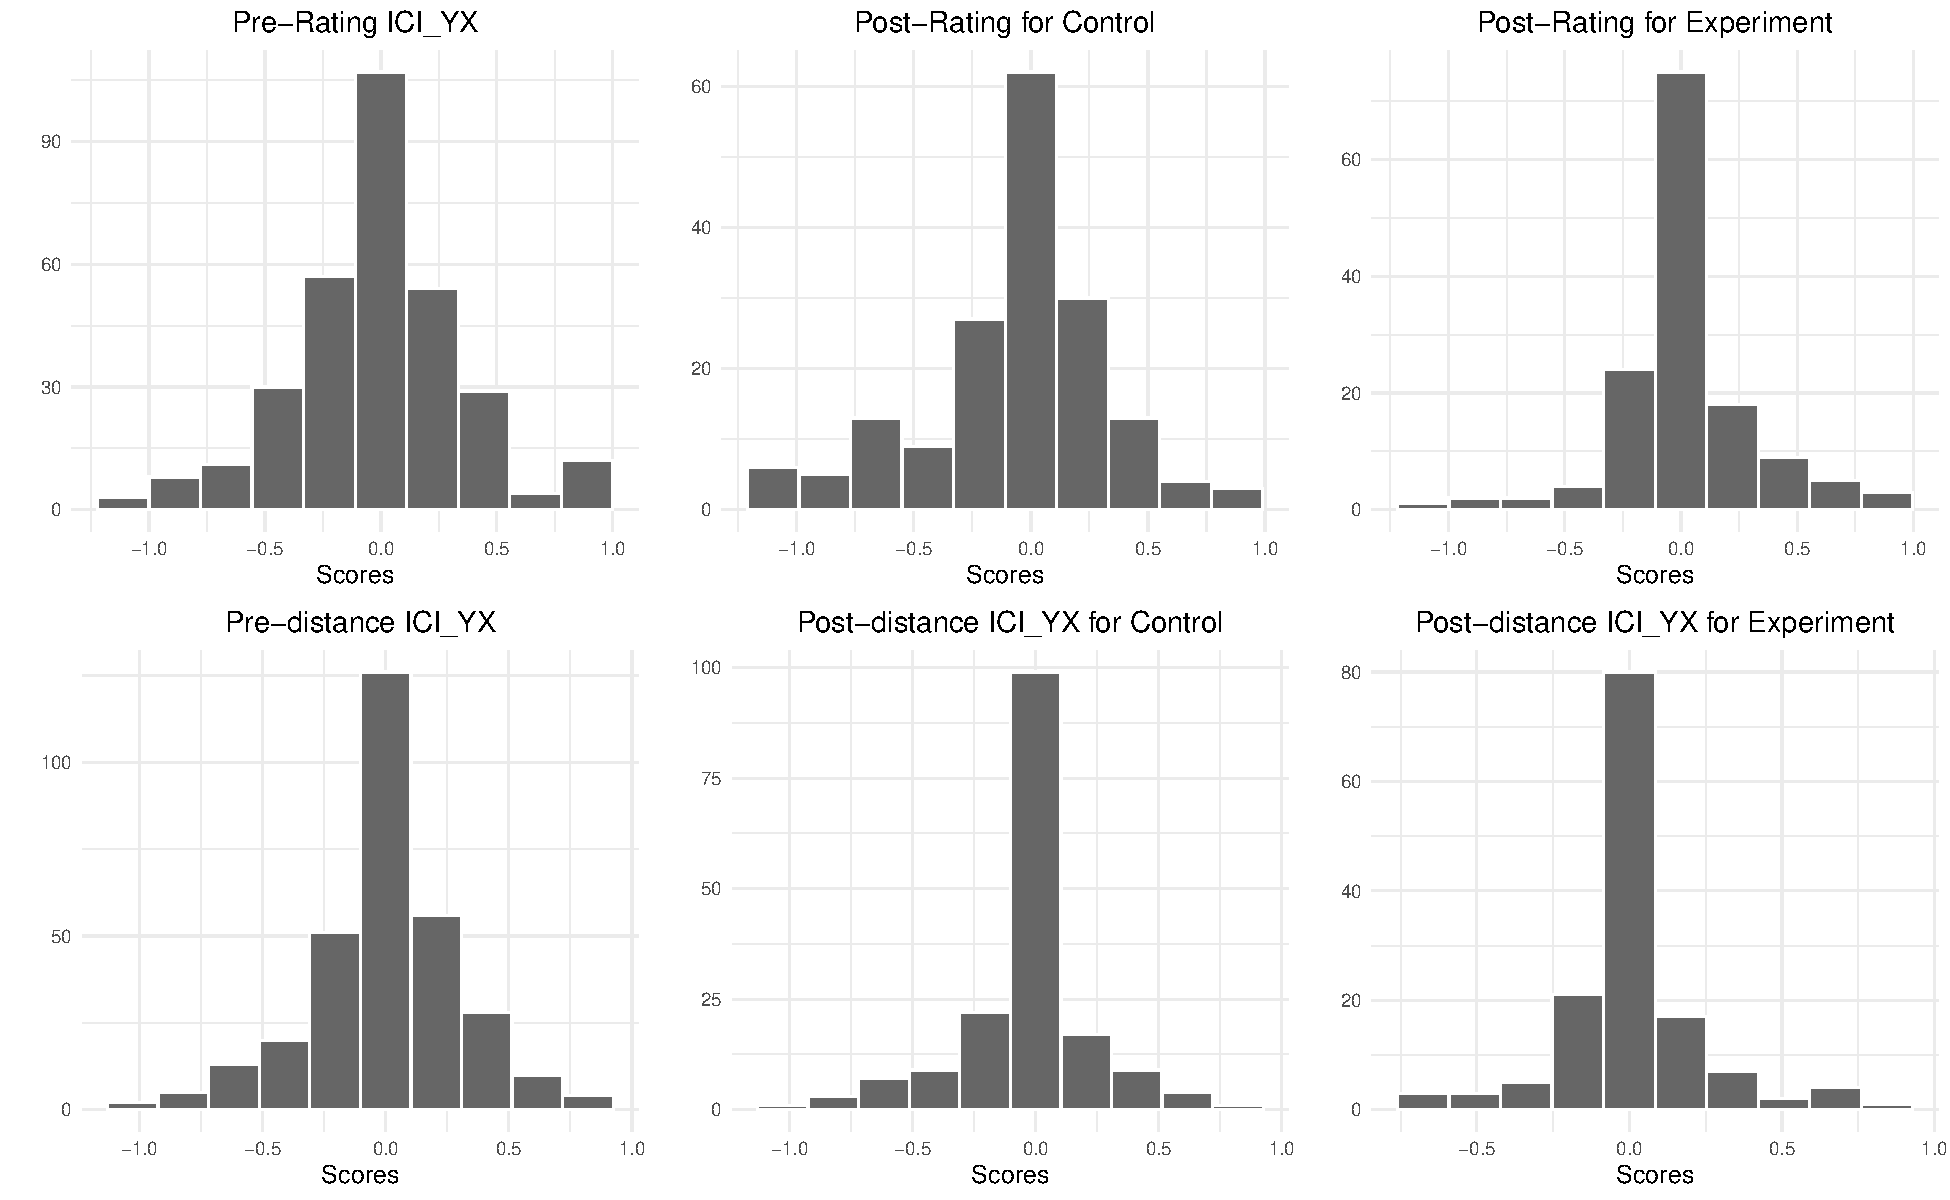
\includegraphics{index_files/figure-pdf/unnamed-chunk-19-1.pdf}

\begin{Shaded}
\begin{Highlighting}[]
\NormalTok{p1 }\OtherTok{\textless{}{-}} \FunctionTok{plot\_distribution}\NormalTok{(df\_prp\_both, }\StringTok{"ICI\_WZ\_rating\_pre\_norm"}\NormalTok{, }\StringTok{"Pre{-}Rating ICI\_WZ"}\NormalTok{)}

\NormalTok{p4 }\OtherTok{\textless{}{-}} \FunctionTok{plot\_distribution}\NormalTok{(df\_prp\_both, }\StringTok{"ICI\_WZ\_dist\_pre\_norm"}\NormalTok{, }\StringTok{"Pre{-}distance ICI\_WZ"}\NormalTok{)}

\FunctionTok{grid.arrange}\NormalTok{(p1, p4, }\AttributeTok{ncol =} \DecValTok{2}\NormalTok{)}
\end{Highlighting}
\end{Shaded}

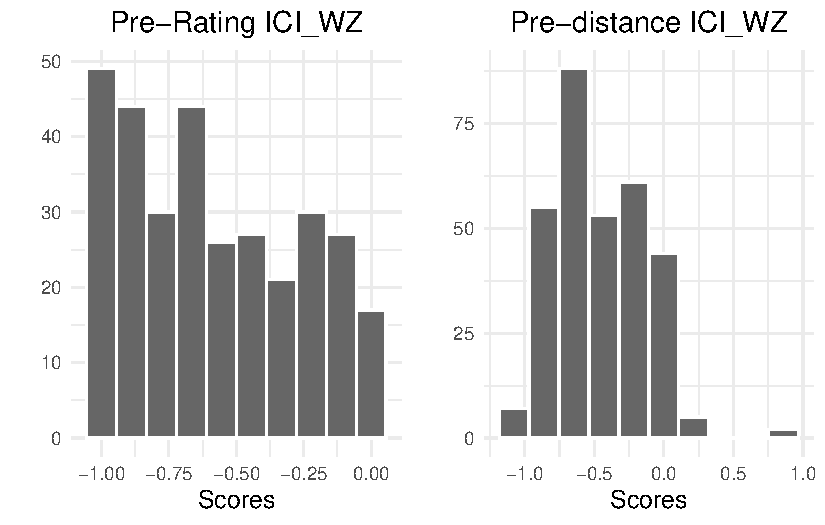
\includegraphics{index_files/figure-pdf/unnamed-chunk-20-1.pdf}

\begin{Shaded}
\begin{Highlighting}[]
\CommentTok{\# First plot: Scatter plot of ICI\_YX\_rating\_pre\_norm vs ICI\_WZ\_rating\_pre\_norm}
\FunctionTok{ggplot}\NormalTok{(df\_prp\_both, }\FunctionTok{aes}\NormalTok{(}\AttributeTok{x =}\NormalTok{ ICI\_YX\_rating\_pre\_norm, }\AttributeTok{y =}\NormalTok{ ICI\_WZ\_rating\_pre\_norm)) }\SpecialCharTok{+}
  \FunctionTok{geom\_point}\NormalTok{() }\SpecialCharTok{+}
  \FunctionTok{labs}\NormalTok{(}\AttributeTok{title =} \StringTok{"Scatter plot of ICI\_YX vs ICI\_WZ Ratings"}\NormalTok{,}
       \AttributeTok{x =} \StringTok{"ICI\_YX Rating"}\NormalTok{,}
       \AttributeTok{y =} \StringTok{"ICI\_WZ Rating"}\NormalTok{) }\SpecialCharTok{+}
  \FunctionTok{theme\_minimal}\NormalTok{()}
\end{Highlighting}
\end{Shaded}

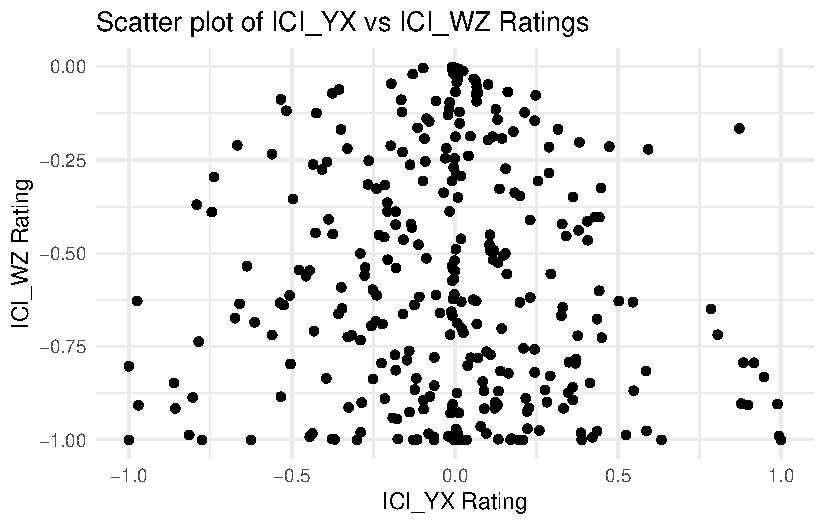
\includegraphics{index_files/figure-pdf/unnamed-chunk-21-1.pdf}

\begin{Shaded}
\begin{Highlighting}[]
\CommentTok{\# Second plot: Scatter plot of ICI\_YX\_dist\_pre\_norm vs ICI\_WZ\_dist\_pre\_norm}
\FunctionTok{ggplot}\NormalTok{(df\_prp\_both, }\FunctionTok{aes}\NormalTok{(}\AttributeTok{x =}\NormalTok{ ICI\_YX\_dist\_pre\_norm, }\AttributeTok{y =}\NormalTok{ ICI\_WZ\_dist\_pre\_norm)) }\SpecialCharTok{+}
  \FunctionTok{geom\_point}\NormalTok{() }\SpecialCharTok{+}
  \FunctionTok{labs}\NormalTok{(}\AttributeTok{title =} \StringTok{"Scatter plot of ICI\_YX vs ICI\_WZ Distances"}\NormalTok{,}
       \AttributeTok{x =} \StringTok{"ICI\_YX Distance"}\NormalTok{,}
       \AttributeTok{y =} \StringTok{"ICI\_WZ Distance"}\NormalTok{) }\SpecialCharTok{+}
  \FunctionTok{theme\_minimal}\NormalTok{()}
\end{Highlighting}
\end{Shaded}

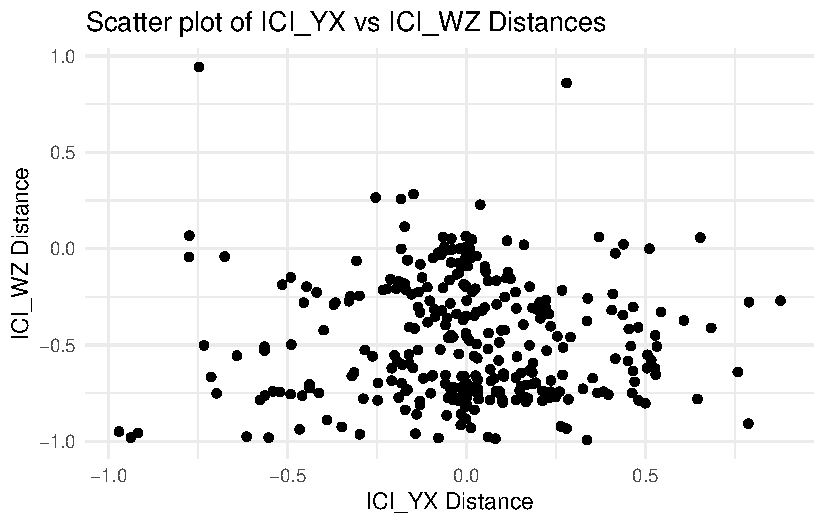
\includegraphics{index_files/figure-pdf/unnamed-chunk-21-2.pdf}

Plot accumulated probability distribution group by stimulus type

\begin{Shaded}
\begin{Highlighting}[]
\NormalTok{plot\_accumulated\_density }\OtherTok{\textless{}{-}} \ControlFlowTok{function}\NormalTok{(df, x, color, title) \{}
\NormalTok{  p }\OtherTok{\textless{}{-}} \FunctionTok{ggplot}\NormalTok{(df, }\FunctionTok{aes}\NormalTok{(}\AttributeTok{x =} \SpecialCharTok{!!}\FunctionTok{sym}\NormalTok{(x), }\AttributeTok{color =} \SpecialCharTok{!!}\FunctionTok{sym}\NormalTok{(color))) }\SpecialCharTok{+}
    \FunctionTok{stat\_ecdf}\NormalTok{(}\AttributeTok{geom =} \StringTok{"step"}\NormalTok{, }\AttributeTok{size =} \DecValTok{1}\NormalTok{) }\SpecialCharTok{+}  
    \FunctionTok{labs}\NormalTok{(}\AttributeTok{title =}\NormalTok{ title, }\AttributeTok{x =} \StringTok{"Scores"}\NormalTok{, }\AttributeTok{y =} \StringTok{"Cumulative Probability"}\NormalTok{) }\SpecialCharTok{+}
    \FunctionTok{theme\_minimal}\NormalTok{() }\SpecialCharTok{+}
    \FunctionTok{theme}\NormalTok{(}
      \AttributeTok{plot.title =} \FunctionTok{element\_text}\NormalTok{(}\AttributeTok{size =} \DecValTok{14}\NormalTok{, }\AttributeTok{hjust =} \FloatTok{0.5}\NormalTok{),}
      \AttributeTok{axis.title.x =} \FunctionTok{element\_text}\NormalTok{(}\AttributeTok{size =} \DecValTok{12}\NormalTok{),}
      \AttributeTok{axis.title.y =} \FunctionTok{element\_text}\NormalTok{(}\AttributeTok{size =} \DecValTok{12}\NormalTok{)}
\NormalTok{    )}
  \FunctionTok{return}\NormalTok{(p)}
\NormalTok{\}}

\NormalTok{plot\_density }\OtherTok{\textless{}{-}} \ControlFlowTok{function}\NormalTok{(df, x, color, title) \{}
\NormalTok{  p }\OtherTok{\textless{}{-}} \FunctionTok{ggplot}\NormalTok{(df, }\FunctionTok{aes}\NormalTok{(}\AttributeTok{x =} \SpecialCharTok{!!}\FunctionTok{sym}\NormalTok{(x), }\AttributeTok{color =} \SpecialCharTok{!!}\FunctionTok{sym}\NormalTok{(color))) }\SpecialCharTok{+}
    \FunctionTok{geom\_density}\NormalTok{(}\FunctionTok{aes}\NormalTok{(}\AttributeTok{y =}\NormalTok{ ..count..), }\AttributeTok{fill =} \StringTok{"grey40"}\NormalTok{, }\AttributeTok{alpha =} \FloatTok{0.5}\NormalTok{) }\SpecialCharTok{+}
    \CommentTok{\#stat\_ecdf(geom = "step", size = 1) +  }
    \FunctionTok{labs}\NormalTok{(}\AttributeTok{title =}\NormalTok{ title, }\AttributeTok{x =} \StringTok{"Scores"}\NormalTok{, }\AttributeTok{y =} \StringTok{"Cumulative Probability"}\NormalTok{) }\SpecialCharTok{+}
    \FunctionTok{theme\_minimal}\NormalTok{() }\SpecialCharTok{+}
    \FunctionTok{theme}\NormalTok{(}
      \AttributeTok{plot.title =} \FunctionTok{element\_text}\NormalTok{(}\AttributeTok{size =} \DecValTok{14}\NormalTok{, }\AttributeTok{hjust =} \FloatTok{0.5}\NormalTok{),}
      \AttributeTok{axis.title.x =} \FunctionTok{element\_text}\NormalTok{(}\AttributeTok{size =} \DecValTok{12}\NormalTok{),}
      \AttributeTok{axis.title.y =} \FunctionTok{element\_text}\NormalTok{(}\AttributeTok{size =} \DecValTok{12}\NormalTok{)}
\NormalTok{    )}
  \FunctionTok{return}\NormalTok{(p)}
\NormalTok{\}}
\end{Highlighting}
\end{Shaded}

\begin{Shaded}
\begin{Highlighting}[]
\NormalTok{p1 }\OtherTok{\textless{}{-}} \FunctionTok{plot\_density}\NormalTok{(df\_prp\_both, }\StringTok{"ICI\_YX\_rating\_pre\_norm"}\NormalTok{, }\StringTok{"stimulus\_type\_X\_Y"}\NormalTok{, }\StringTok{"Density}\SpecialCharTok{\textbackslash{}n}\StringTok{ of Pre{-}Rating"}\NormalTok{)}
\NormalTok{p2 }\OtherTok{\textless{}{-}} \FunctionTok{plot\_density}\NormalTok{(df\_prp\_both, }\StringTok{"ICI\_YX\_dist\_pre\_norm"}\NormalTok{, }\StringTok{"stimulus\_type\_X\_Y"}\NormalTok{, }\StringTok{"Density }\SpecialCharTok{\textbackslash{}n}\StringTok{ of Pre{-}Distance"}\NormalTok{)}

\FunctionTok{grid.arrange}\NormalTok{(p1, p2, }\AttributeTok{ncol=}\DecValTok{2}\NormalTok{)}
\end{Highlighting}
\end{Shaded}

\begin{verbatim}
Warning: The dot-dot notation (`..count..`) was deprecated in ggplot2 3.4.0.
i Please use `after_stat(count)` instead.
\end{verbatim}

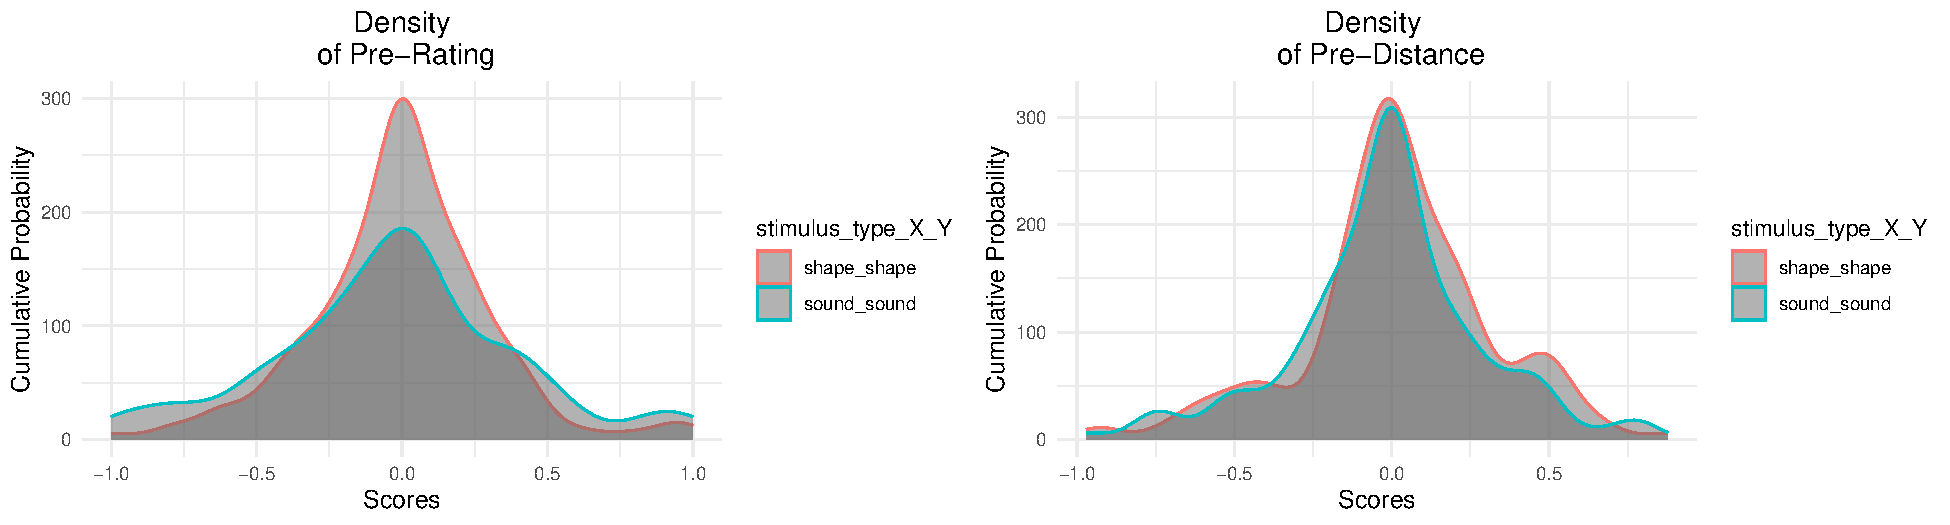
\includegraphics{index_files/figure-pdf/unnamed-chunk-23-1.pdf}

\begin{Shaded}
\begin{Highlighting}[]
\NormalTok{p1 }\OtherTok{\textless{}{-}} \FunctionTok{plot\_accumulated\_density}\NormalTok{(df\_prp\_both, }\StringTok{"ICI\_YX\_rating\_pre\_norm"}\NormalTok{, }\StringTok{"stimulus\_type\_X\_Y"}\NormalTok{, }\StringTok{"Cumulative Density}\SpecialCharTok{\textbackslash{}n}\StringTok{ of Pre{-}Rating"}\NormalTok{)}
\end{Highlighting}
\end{Shaded}

\begin{verbatim}
Warning: Using `size` aesthetic for lines was deprecated in ggplot2 3.4.0.
i Please use `linewidth` instead.
\end{verbatim}

\begin{Shaded}
\begin{Highlighting}[]
\NormalTok{p2 }\OtherTok{\textless{}{-}} \FunctionTok{plot\_accumulated\_density}\NormalTok{(df\_prp\_both, }\StringTok{"ICI\_YX\_dist\_pre\_norm"}\NormalTok{, }\StringTok{"stimulus\_type\_X\_Y"}\NormalTok{, }\StringTok{"Cumulative Density }\SpecialCharTok{\textbackslash{}n}\StringTok{ of Pre{-}Distance"}\NormalTok{)}

\FunctionTok{grid.arrange}\NormalTok{(p1, p2, }\AttributeTok{ncol=}\DecValTok{2}\NormalTok{)}
\end{Highlighting}
\end{Shaded}

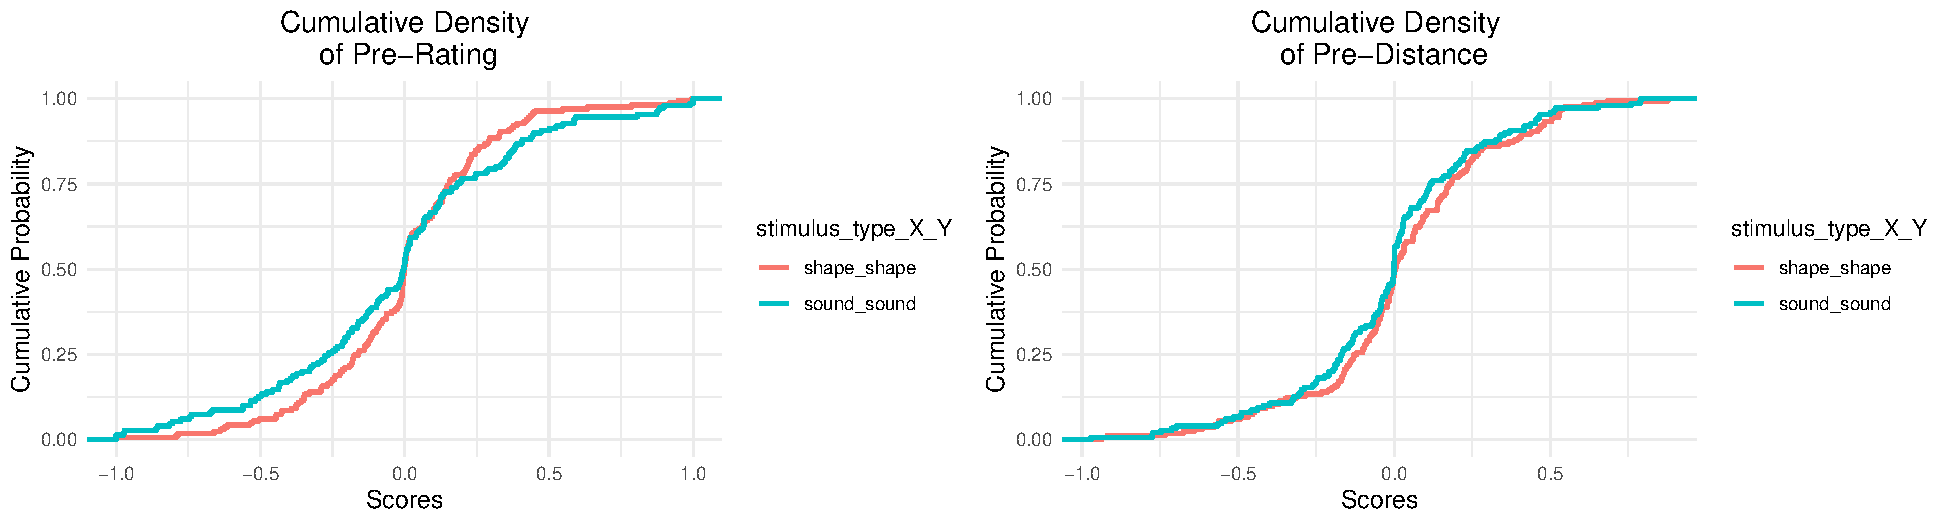
\includegraphics{index_files/figure-pdf/unnamed-chunk-24-1.pdf}

\begin{Shaded}
\begin{Highlighting}[]
\NormalTok{p1 }\OtherTok{\textless{}{-}} \FunctionTok{plot\_density}\NormalTok{(df\_prp\_both, }\StringTok{"ICI\_YX\_rating\_pre\_norm"}\NormalTok{, }\StringTok{"stimulus\_X\_Y"}\NormalTok{, }\StringTok{"Density of Pre{-}Rating"}\NormalTok{)}

\FunctionTok{grid.arrange}\NormalTok{(p1, }\AttributeTok{ncol=}\DecValTok{1}\NormalTok{)}
\end{Highlighting}
\end{Shaded}

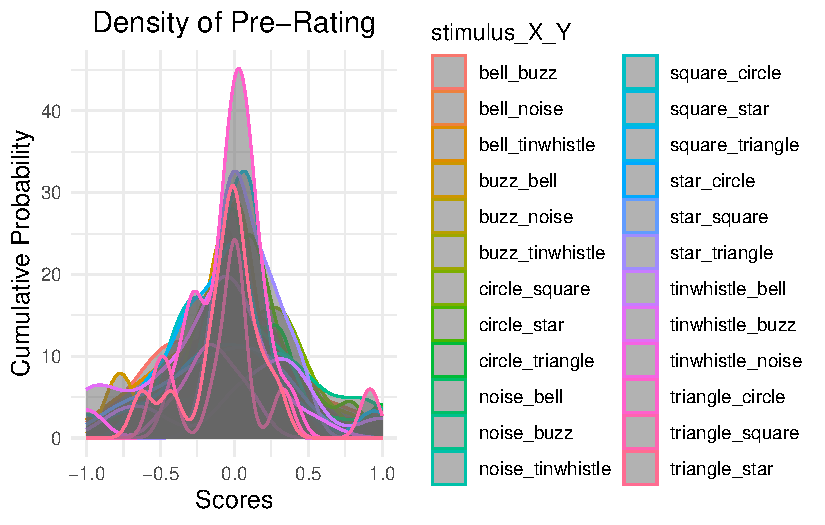
\includegraphics{index_files/figure-pdf/unnamed-chunk-25-1.pdf}

\begin{Shaded}
\begin{Highlighting}[]
\NormalTok{p1 }\OtherTok{\textless{}{-}} \FunctionTok{plot\_density}\NormalTok{(df\_prp\_both, }\StringTok{"ICI\_YX\_dist\_pre\_norm"}\NormalTok{, }\StringTok{"stimulus\_X\_Y"}\NormalTok{, }\StringTok{"Density of Pre{-}Distance"}\NormalTok{)}

\FunctionTok{grid.arrange}\NormalTok{(p1, }\AttributeTok{ncol=}\DecValTok{1}\NormalTok{)}
\end{Highlighting}
\end{Shaded}

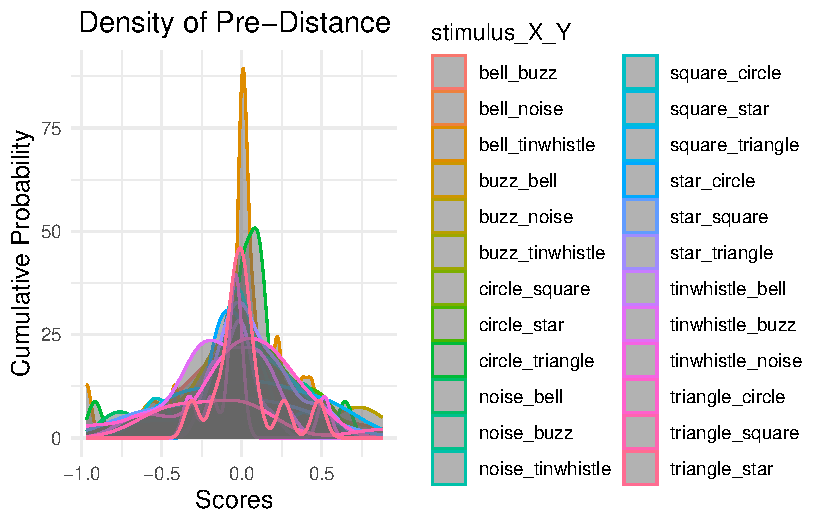
\includegraphics{index_files/figure-pdf/unnamed-chunk-25-2.pdf}

\begin{Shaded}
\begin{Highlighting}[]
\NormalTok{p1 }\OtherTok{\textless{}{-}} \FunctionTok{plot\_accumulated\_density}\NormalTok{(df\_prp\_both, }\StringTok{"ICI\_YX\_rating\_pre\_norm"}\NormalTok{, }\StringTok{"stimulus\_X\_Y"}\NormalTok{, }\StringTok{"Cumulative Density of Pre{-}Rating"}\NormalTok{)}

\FunctionTok{grid.arrange}\NormalTok{(p1, }\AttributeTok{ncol=}\DecValTok{1}\NormalTok{)}
\end{Highlighting}
\end{Shaded}

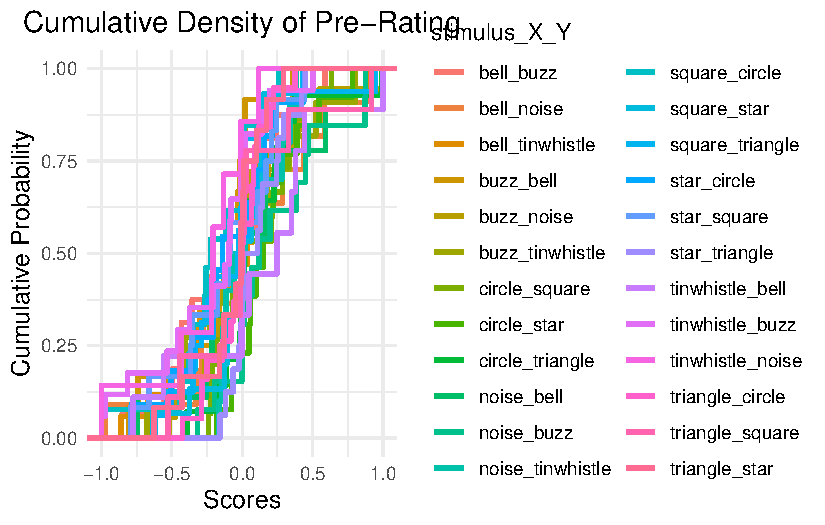
\includegraphics{index_files/figure-pdf/unnamed-chunk-26-1.pdf}

\begin{Shaded}
\begin{Highlighting}[]
\NormalTok{p1 }\OtherTok{\textless{}{-}} \FunctionTok{plot\_accumulated\_density}\NormalTok{(df\_prp\_both, }\StringTok{"ICI\_YX\_dist\_pre\_norm"}\NormalTok{, }\StringTok{"stimulus\_X\_Y"}\NormalTok{, }\StringTok{"Cumulative Density of Pre{-}Distance"}\NormalTok{)}

\FunctionTok{grid.arrange}\NormalTok{(p1, }\AttributeTok{ncol=}\DecValTok{1}\NormalTok{)}
\end{Highlighting}
\end{Shaded}

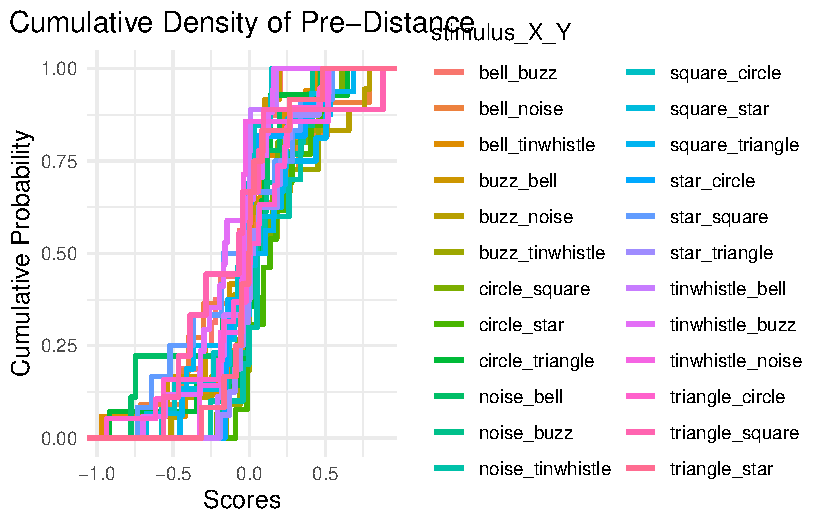
\includegraphics{index_files/figure-pdf/unnamed-chunk-26-2.pdf}

\subsubsection{One-way ANOVA test for normalized pre-manipulation
indexes with stimulus
type}\label{one-way-anova-test-for-normalized-pre-manipulation-indexes-with-stimulus-type}

\begin{Shaded}
\begin{Highlighting}[]
\FunctionTok{summary}\NormalTok{(}\FunctionTok{aov}\NormalTok{(df\_prp\_both}\SpecialCharTok{$}\NormalTok{ICI\_YX\_rating\_pre\_norm }\SpecialCharTok{\textasciitilde{}}\NormalTok{ df\_prp\_both}\SpecialCharTok{$}\NormalTok{stimulus\_type\_X\_Y))}
\end{Highlighting}
\end{Shaded}

\begin{verbatim}
                               Df Sum Sq Mean Sq F value Pr(>F)
df_prp_both$stimulus_type_X_Y   1   0.05 0.04751   0.358   0.55
Residuals                     313  41.48 0.13254               
\end{verbatim}

\begin{Shaded}
\begin{Highlighting}[]
\FunctionTok{summary}\NormalTok{(}\FunctionTok{aov}\NormalTok{(df\_prp\_both}\SpecialCharTok{$}\NormalTok{ICI\_YX\_dist\_pre\_norm }\SpecialCharTok{\textasciitilde{}}\NormalTok{ df\_prp\_both}\SpecialCharTok{$}\NormalTok{stimulus\_type\_X\_Y))}
\end{Highlighting}
\end{Shaded}

\begin{verbatim}
                               Df Sum Sq Mean Sq F value Pr(>F)
df_prp_both$stimulus_type_X_Y   1  0.092 0.09172   1.008  0.316
Residuals                     313 28.489 0.09102               
\end{verbatim}

\subsubsection{Normality test}\label{normality-test}

Test for normality using Shapiro-Wilk Test for each index. They seems
normal.

\begin{Shaded}
\begin{Highlighting}[]
\FunctionTok{shapiro.test}\NormalTok{(df\_prp\_both}\SpecialCharTok{$}\NormalTok{ICI\_YX\_rating\_pre\_norm)}
\end{Highlighting}
\end{Shaded}

\begin{verbatim}

    Shapiro-Wilk normality test

data:  df_prp_both$ICI_YX_rating_pre_norm
W = 0.97394, p-value = 1.777e-05
\end{verbatim}

\begin{Shaded}
\begin{Highlighting}[]
\FunctionTok{shapiro.test}\NormalTok{(df\_prp\_both}\SpecialCharTok{$}\NormalTok{ICI\_YX\_dist\_pre\_norm)}
\end{Highlighting}
\end{Shaded}

\begin{verbatim}

    Shapiro-Wilk normality test

data:  df_prp_both$ICI_YX_dist_pre_norm
W = 0.9726, p-value = 1.056e-05
\end{verbatim}

\begin{Shaded}
\begin{Highlighting}[]
\FunctionTok{shapiro.test}\NormalTok{(df\_prp\_both}\SpecialCharTok{$}\NormalTok{ICI\_YX\_rating\_post\_norm)}
\end{Highlighting}
\end{Shaded}

\begin{verbatim}

    Shapiro-Wilk normality test

data:  df_prp_both$ICI_YX_rating_post_norm
W = 0.93783, p-value = 3.192e-10
\end{verbatim}

\begin{Shaded}
\begin{Highlighting}[]
\FunctionTok{shapiro.test}\NormalTok{(df\_prp\_both}\SpecialCharTok{$}\NormalTok{ICI\_YX\_dist\_post\_norm)}
\end{Highlighting}
\end{Shaded}

\begin{verbatim}

    Shapiro-Wilk normality test

data:  df_prp_both$ICI_YX_dist_post_norm
W = 0.88533, p-value = 1.257e-14
\end{verbatim}

\subsubsection{Correlations}\label{correlations}

\begin{Shaded}
\begin{Highlighting}[]
\NormalTok{df\_shorted\_name }\OtherTok{\textless{}{-}}\NormalTok{ df\_prp\_both }\SpecialCharTok{\%\textgreater{}\%}
  \FunctionTok{mutate}\NormalTok{(}\AttributeTok{rating\_pre =}\NormalTok{ ICI\_YX\_rating\_pre\_norm,}
         \AttributeTok{rating\_post =}\NormalTok{ ICI\_YX\_rating\_post\_norm,}
         \AttributeTok{distance\_pre =}\NormalTok{ ICI\_YX\_dist\_pre\_norm,}
         \AttributeTok{distance\_post =}\NormalTok{ ICI\_YX\_dist\_post\_norm)}
  
\NormalTok{selected\_columns }\OtherTok{\textless{}{-}}\NormalTok{ df\_shorted\_name[, }\FunctionTok{c}\NormalTok{(}\StringTok{\textquotesingle{}anxiety\textquotesingle{}}\NormalTok{, }\StringTok{\textquotesingle{}stress\textquotesingle{}}\NormalTok{, }\StringTok{\textquotesingle{}depression\textquotesingle{}}\NormalTok{, }\StringTok{\textquotesingle{}Sex\_0\textquotesingle{}}\NormalTok{, }\StringTok{\textquotesingle{}age\textquotesingle{}}\NormalTok{, }\StringTok{\textquotesingle{}rating\_pre\textquotesingle{}}\NormalTok{, }\StringTok{\textquotesingle{}rating\_post\textquotesingle{}}\NormalTok{, }\StringTok{\textquotesingle{}distance\_pre\textquotesingle{}}\NormalTok{, }\StringTok{\textquotesingle{}distance\_post\textquotesingle{}}\NormalTok{)]}

\NormalTok{cor\_matrix }\OtherTok{\textless{}{-}} \FunctionTok{cor}\NormalTok{(selected\_columns, }\AttributeTok{use =} \StringTok{"complete.obs"}\NormalTok{)}
\NormalTok{cor\_matrix}
\end{Highlighting}
\end{Shaded}

\begin{verbatim}
                  anxiety      stress  depression        Sex_0         age
anxiety        1.00000000  0.84290961  0.84950350  0.013009678 -0.19038253
stress         0.84290961  1.00000000  0.85358218  0.077319077 -0.22205455
depression     0.84950350  0.85358218  1.00000000  0.083863705 -0.18094134
Sex_0          0.01300968  0.07731908  0.08386371  1.000000000  0.07366257
age           -0.19038253 -0.22205455 -0.18094134  0.073662574  1.00000000
rating_pre    -0.07560735 -0.07443259 -0.06005502  0.049078888  0.04878348
rating_post   -0.03295682 -0.02751596 -0.02375800 -0.004242396 -0.08268928
distance_pre  -0.10107376 -0.11389789 -0.09086615  0.072636159  0.04887542
distance_post -0.03164209 -0.02601200 -0.02175057 -0.075899821 -0.12185594
               rating_pre  rating_post distance_pre distance_post
anxiety       -0.07560735 -0.032956823  -0.10107376   -0.03164209
stress        -0.07443259 -0.027515956  -0.11389789   -0.02601200
depression    -0.06005502 -0.023758000  -0.09086615   -0.02175057
Sex_0          0.04907889 -0.004242396   0.07263616   -0.07589982
age            0.04878348 -0.082689278   0.04887542   -0.12185594
rating_pre     1.00000000  0.309718470   0.55006694    0.29041970
rating_post    0.30971847  1.000000000   0.33540380    0.59092254
distance_pre   0.55006694  0.335403797   1.00000000    0.31594470
distance_post  0.29041970  0.590922542   0.31594470    1.00000000
\end{verbatim}

\begin{Shaded}
\begin{Highlighting}[]
\CommentTok{\# Plot the heatmap using corrplot}
\FunctionTok{corrplot}\NormalTok{(cor\_matrix, }\AttributeTok{method =} \StringTok{"color"}\NormalTok{, }\AttributeTok{tl.col =} \StringTok{"black"}\NormalTok{, }\AttributeTok{tl.srt =} \DecValTok{45}\NormalTok{, }
         \AttributeTok{addCoef.col =} \StringTok{"black"}\NormalTok{, }\AttributeTok{number.cex =} \FloatTok{0.7}\NormalTok{, }\AttributeTok{col =} \FunctionTok{colorRampPalette}\NormalTok{(}\FunctionTok{c}\NormalTok{(}\StringTok{"blue"}\NormalTok{, }\StringTok{"white"}\NormalTok{, }\StringTok{"red"}\NormalTok{))(}\DecValTok{200}\NormalTok{),}
         \AttributeTok{title =} \StringTok{"Correlation Heatmap"}\NormalTok{, }\AttributeTok{mar =} \FunctionTok{c}\NormalTok{(}\DecValTok{0}\NormalTok{, }\DecValTok{0}\NormalTok{, }\DecValTok{1}\NormalTok{, }\DecValTok{0}\NormalTok{))}
\end{Highlighting}
\end{Shaded}

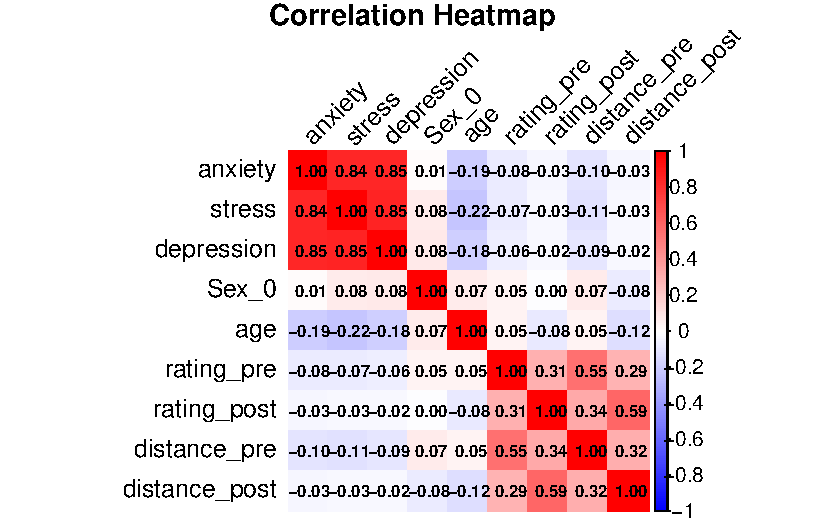
\includegraphics{index_files/figure-pdf/unnamed-chunk-31-1.pdf}

Calculate p-values for the correlation matrix

\begin{Shaded}
\begin{Highlighting}[]
\NormalTok{vars }\OtherTok{\textless{}{-}} \FunctionTok{names}\NormalTok{(selected\_columns)}
\NormalTok{n }\OtherTok{\textless{}{-}} \FunctionTok{length}\NormalTok{(vars)}
\NormalTok{p\_matrix }\OtherTok{\textless{}{-}} \FunctionTok{matrix}\NormalTok{(}\ConstantTok{NA}\NormalTok{, n, n)}
\FunctionTok{colnames}\NormalTok{(p\_matrix) }\OtherTok{\textless{}{-}} \FunctionTok{rownames}\NormalTok{(p\_matrix) }\OtherTok{\textless{}{-}}\NormalTok{ vars}

\ControlFlowTok{for}\NormalTok{ (i }\ControlFlowTok{in} \DecValTok{1}\SpecialCharTok{:}\NormalTok{n) \{}
  \ControlFlowTok{for}\NormalTok{ (j }\ControlFlowTok{in} \DecValTok{1}\SpecialCharTok{:}\NormalTok{n) \{}
\NormalTok{    test }\OtherTok{\textless{}{-}} \FunctionTok{cor.test}\NormalTok{(selected\_columns[[i]], selected\_columns[[j]], }\AttributeTok{method =} \StringTok{"pearson"}\NormalTok{)}
\NormalTok{    p\_matrix[i, j] }\OtherTok{\textless{}{-}}\NormalTok{ test}\SpecialCharTok{$}\NormalTok{p.value}
\NormalTok{  \}}
\NormalTok{\}}
\NormalTok{p\_matrix}
\end{Highlighting}
\end{Shaded}

\begin{verbatim}
                   anxiety       stress   depression     Sex_0          age
anxiety       0.000000e+00 2.994172e-86 6.326143e-89 0.8180990 6.821868e-04
stress        2.994172e-86 0.000000e+00 1.206063e-90 0.1710393 7.033532e-05
depression    6.326143e-89 1.206063e-90 0.000000e+00 0.1375086 1.258470e-03
Sex_0         8.180990e-01 1.710393e-01 1.375086e-01 0.0000000 1.922487e-01
age           6.821868e-04 7.033532e-05 1.258470e-03 0.1922487 0.000000e+00
rating_pre    1.807403e-01 1.876295e-01 2.879666e-01 0.3853263 3.881965e-01
rating_post   5.600559e-01 6.266053e-01 6.744521e-01 0.9402179 1.431220e-01
distance_pre  7.323881e-02 4.338042e-02 1.074777e-01 0.1985346 3.873018e-01
distance_post 5.758213e-01 6.455810e-01 7.005745e-01 0.1790546 3.060322e-02
                rating_pre  rating_post distance_pre distance_post
anxiety       1.807403e-01 5.600559e-01 7.323881e-02  5.758213e-01
stress        1.876295e-01 6.266053e-01 4.338042e-02  6.455810e-01
depression    2.879666e-01 6.744521e-01 1.074777e-01  7.005745e-01
Sex_0         3.853263e-01 9.402179e-01 1.985346e-01  1.790546e-01
age           3.881965e-01 1.431220e-01 3.873018e-01  3.060322e-02
rating_pre    0.000000e+00 1.980002e-08 2.616836e-26  1.541963e-07
rating_post   1.980002e-08 0.000000e+00 1.015451e-09  4.846184e-31
distance_pre  2.616836e-26 1.015451e-09 0.000000e+00  9.886029e-09
distance_post 1.541963e-07 4.846184e-31 9.886029e-09  0.000000e+00
\end{verbatim}

\subsubsection{Assign styles}\label{assign-styles}

Segment the participants into three groups based on their
pre-manipulation ratings and distances.

\begin{Shaded}
\begin{Highlighting}[]
\CommentTok{\# Calculate the SD for Pre and define participants\textquotesingle{} styles}
\NormalTok{rating\_quantile }\OtherTok{\textless{}{-}} \FunctionTok{quantile}\NormalTok{(df\_prp\_both}\SpecialCharTok{$}\NormalTok{ICI\_YX\_rating\_pre\_norm, }\FunctionTok{c}\NormalTok{(}\DecValTok{1}\SpecialCharTok{/}\DecValTok{3}\NormalTok{, }\DecValTok{2}\SpecialCharTok{/}\DecValTok{3}\NormalTok{))}
\NormalTok{dist\_quantile }\OtherTok{\textless{}{-}} \FunctionTok{quantile}\NormalTok{(df\_prp\_both}\SpecialCharTok{$}\NormalTok{ICI\_YX\_dist\_pre\_norm, }\FunctionTok{c}\NormalTok{(}\DecValTok{1}\SpecialCharTok{/}\DecValTok{3}\NormalTok{, }\DecValTok{2}\SpecialCharTok{/}\DecValTok{3}\NormalTok{))}

\NormalTok{df\_prp\_both }\OtherTok{\textless{}{-}}\NormalTok{ df\_prp\_both }\SpecialCharTok{\%\textgreater{}\%}
  \FunctionTok{mutate}\NormalTok{(}\CommentTok{\# rating}
         \AttributeTok{sd\_pre\_rating =} \FunctionTok{sd}\NormalTok{(ICI\_YX\_rating\_pre\_norm, }\AttributeTok{na.rm =} \ConstantTok{TRUE}\NormalTok{),}
         \AttributeTok{mean\_pre\_rating =} \FunctionTok{mean}\NormalTok{(ICI\_YX\_rating\_pre\_norm, }\AttributeTok{na.rm =} \ConstantTok{TRUE}\NormalTok{),}
         \AttributeTok{style\_rating =} \FunctionTok{case\_when}\NormalTok{(}
           \CommentTok{\#ICI\_YX\_rating\_pre\_norm \textgreater{} mean\_pre\_rating + sd\_pre\_rating \textasciitilde{} "Competitive",}
           \CommentTok{\#ICI\_YX\_rating\_pre\_norm \textless{} mean\_pre\_rating {-} sd\_pre\_rating \textasciitilde{} "Facilitative",}
\NormalTok{           ICI\_YX\_rating\_pre\_norm }\SpecialCharTok{\textgreater{}}\NormalTok{ rating\_quantile[}\DecValTok{2}\NormalTok{] }\SpecialCharTok{\textasciitilde{}} \StringTok{"Competitive"}\NormalTok{,}
\NormalTok{           ICI\_YX\_rating\_pre\_norm }\SpecialCharTok{\textless{}}\NormalTok{ rating\_quantile[}\DecValTok{1}\NormalTok{] }\SpecialCharTok{\textasciitilde{}} \StringTok{"Facilitative"}\NormalTok{,}
           \AttributeTok{.default =} \StringTok{"No{-}Difference"}
\NormalTok{         ),}
         \CommentTok{\# distance}
         \AttributeTok{sd\_pre\_distance =} \FunctionTok{sd}\NormalTok{(ICI\_YX\_dist\_pre\_norm, }\AttributeTok{na.rm =} \ConstantTok{TRUE}\NormalTok{),}
         \AttributeTok{mean\_pre\_distance =} \FunctionTok{mean}\NormalTok{(ICI\_YX\_dist\_pre\_norm, }\AttributeTok{na.rm =} \ConstantTok{TRUE}\NormalTok{),}
         \AttributeTok{style\_distance =} \FunctionTok{case\_when}\NormalTok{(}
           \CommentTok{\#ICI\_YX\_dist\_pre\_norm \textgreater{} mean\_pre\_distance + sd\_pre\_distance \textasciitilde{} "Competitive",}
           \CommentTok{\#ICI\_YX\_dist\_pre\_norm \textless{} mean\_pre\_distance {-} sd\_pre\_distance \textasciitilde{} "Facilitative",}
\NormalTok{           ICI\_YX\_dist\_pre\_norm }\SpecialCharTok{\textgreater{}}\NormalTok{ dist\_quantile[}\DecValTok{2}\NormalTok{] }\SpecialCharTok{\textasciitilde{}} \StringTok{"Competitive"}\NormalTok{,}
\NormalTok{           ICI\_YX\_dist\_pre\_norm }\SpecialCharTok{\textless{}}\NormalTok{ dist\_quantile[}\DecValTok{1}\NormalTok{] }\SpecialCharTok{\textasciitilde{}} \StringTok{"Facilitative"}\NormalTok{,}
           \AttributeTok{.default =} \StringTok{"No{-}Difference"}
\NormalTok{         ))}
\end{Highlighting}
\end{Shaded}

How many participants in each style?

\begin{Shaded}
\begin{Highlighting}[]
\NormalTok{df\_prp\_both }\SpecialCharTok{\%\textgreater{}\%}
  \FunctionTok{group\_by}\NormalTok{(style\_rating) }\SpecialCharTok{\%\textgreater{}\%}
  \FunctionTok{summarize}\NormalTok{(}\AttributeTok{n =} \FunctionTok{n\_distinct}\NormalTok{(subjectID))}
\end{Highlighting}
\end{Shaded}

\begin{verbatim}
# A tibble: 3 x 2
  style_rating      n
  <chr>         <int>
1 Competitive     105
2 Facilitative    105
3 No-Difference   105
\end{verbatim}

\begin{Shaded}
\begin{Highlighting}[]
\NormalTok{df\_prp\_both }\SpecialCharTok{\%\textgreater{}\%}
  \FunctionTok{group\_by}\NormalTok{(style\_distance) }\SpecialCharTok{\%\textgreater{}\%}
  \FunctionTok{summarize}\NormalTok{(}\AttributeTok{n =} \FunctionTok{n\_distinct}\NormalTok{(subjectID))}
\end{Highlighting}
\end{Shaded}

\begin{verbatim}
# A tibble: 3 x 2
  style_distance     n
  <chr>          <int>
1 Competitive      105
2 Facilitative     105
3 No-Difference    105
\end{verbatim}

\subsubsection{One-way ANOVA test for normalized pre-manipulation rating
indexes}\label{one-way-anova-test-for-normalized-pre-manipulation-rating-indexes}

Check assumptions: normality \& homogeneity of variances

\begin{enumerate}
\def\labelenumi{\arabic{enumi}.}
\tightlist
\item
  Shapiro-Wilk (normality within each group)
\end{enumerate}

\begin{Shaded}
\begin{Highlighting}[]
\FunctionTok{by}\NormalTok{(df\_prp\_both}\SpecialCharTok{$}\NormalTok{ICI\_YX\_rating\_pre\_norm, df\_prp\_both}\SpecialCharTok{$}\NormalTok{style\_rating, shapiro.test)}
\end{Highlighting}
\end{Shaded}

\begin{verbatim}
df_prp_both$style_rating: Competitive

    Shapiro-Wilk normality test

data:  dd[x, ]
W = 0.83727, p-value = 2.189e-09

------------------------------------------------------------ 
df_prp_both$style_rating: Facilitative

    Shapiro-Wilk normality test

data:  dd[x, ]
W = 0.88659, p-value = 2.03e-07

------------------------------------------------------------ 
df_prp_both$style_rating: No-Difference

    Shapiro-Wilk normality test

data:  dd[x, ]
W = 0.94961, p-value = 0.0005534
\end{verbatim}

All groups violate the normality assumption, the p-values are all
\textless{} 0.05.

\begin{enumerate}
\def\labelenumi{\arabic{enumi}.}
\setcounter{enumi}{1}
\tightlist
\item
  Levene's test (homogeneity of variance)
\end{enumerate}

\begin{Shaded}
\begin{Highlighting}[]
\NormalTok{df\_prp\_both}\SpecialCharTok{$}\NormalTok{style\_rating\_factor }\OtherTok{\textless{}{-}} \FunctionTok{as.factor}\NormalTok{(df\_prp\_both}\SpecialCharTok{$}\NormalTok{style\_rating)}

\FunctionTok{leveneTest}\NormalTok{(ICI\_YX\_rating\_pre\_norm }\SpecialCharTok{\textasciitilde{}}\NormalTok{ style\_rating\_factor, }\AttributeTok{data =}\NormalTok{ df\_prp\_both)}
\end{Highlighting}
\end{Shaded}

\begin{verbatim}
Levene's Test for Homogeneity of Variance (center = median)
       Df F value   Pr(>F)    
group   2  35.761 1.04e-14 ***
      312                     
---
Signif. codes:  0 '***' 0.001 '**' 0.01 '*' 0.05 '.' 0.1 ' ' 1
\end{verbatim}

The p-value is \textless{} 0.05, indicating that the variances are not
equal across groups.

Run one-way ANOVA

\begin{Shaded}
\begin{Highlighting}[]
\NormalTok{anova\_model }\OtherTok{\textless{}{-}} \FunctionTok{aov}\NormalTok{(ICI\_YX\_rating\_pre\_norm }\SpecialCharTok{\textasciitilde{}}\NormalTok{ style\_rating, }\AttributeTok{data =}\NormalTok{ df\_prp\_both)}
\FunctionTok{summary}\NormalTok{(anova\_model)}
\end{Highlighting}
\end{Shaded}

\begin{verbatim}
              Df Sum Sq Mean Sq F value Pr(>F)    
style_rating   2  29.35  14.677     376 <2e-16 ***
Residuals    312  12.18   0.039                   
---
Signif. codes:  0 '***' 0.001 '**' 0.01 '*' 0.05 '.' 0.1 ' ' 1
\end{verbatim}

\begin{Shaded}
\begin{Highlighting}[]
\FunctionTok{eta\_squared}\NormalTok{(anova\_model)}
\end{Highlighting}
\end{Shaded}

\begin{verbatim}
For one-way between subjects designs, partial eta squared is equivalent
  to eta squared. Returning eta squared.
\end{verbatim}

\begin{verbatim}
# Effect Size for ANOVA

Parameter    | Eta2 |       95% CI
----------------------------------
style_rating | 0.71 | [0.67, 1.00]

- One-sided CIs: upper bound fixed at [1.00].
\end{verbatim}

A one-way between-subjects ANOVA was conducted to examine the effect of
rating style (Competitive, Facilitative, No-Difference) on participants'
normalized pre-manipulation ratings index. The results revealed a
statistically significant effect of rating style on normalized rating
indexes, F(2, 312) = 376.00, p \textless{} .001. The effect size was
large, η² = .71, 95\% CI {[}.67, 1.00{]}, indicating that approximately
71\% of the variance in normalized pre-manipulation rating indexes can
be attributed to rating style.

\subsubsection{One-way ANOVA test for normalized pre-manipulation
distance
indexes}\label{one-way-anova-test-for-normalized-pre-manipulation-distance-indexes}

Check assumptions: normality \& homogeneity of variances

\begin{enumerate}
\def\labelenumi{\arabic{enumi}.}
\tightlist
\item
  Shapiro-Wilk (normality within each group)
\end{enumerate}

\begin{Shaded}
\begin{Highlighting}[]
\FunctionTok{by}\NormalTok{(df\_prp\_both}\SpecialCharTok{$}\NormalTok{ICI\_YX\_dist\_pre\_norm, df\_prp\_both}\SpecialCharTok{$}\NormalTok{style\_distance, shapiro.test)}
\end{Highlighting}
\end{Shaded}

\begin{verbatim}
df_prp_both$style_distance: Competitive

    Shapiro-Wilk normality test

data:  dd[x, ]
W = 0.90653, p-value = 1.776e-06

------------------------------------------------------------ 
df_prp_both$style_distance: Facilitative

    Shapiro-Wilk normality test

data:  dd[x, ]
W = 0.86961, p-value = 3.798e-08

------------------------------------------------------------ 
df_prp_both$style_distance: No-Difference

    Shapiro-Wilk normality test

data:  dd[x, ]
W = 0.96824, p-value = 0.0127
\end{verbatim}

All groups violate the normality assumption, the p-values are all
\textless{} 0.05.

\begin{enumerate}
\def\labelenumi{\arabic{enumi}.}
\setcounter{enumi}{1}
\tightlist
\item
  Levene's test (homogeneity of variance)
\end{enumerate}

\begin{Shaded}
\begin{Highlighting}[]
\NormalTok{df\_prp\_both}\SpecialCharTok{$}\NormalTok{style\_distance\_factor }\OtherTok{\textless{}{-}} \FunctionTok{as.factor}\NormalTok{(df\_prp\_both}\SpecialCharTok{$}\NormalTok{style\_distance)}

\FunctionTok{leveneTest}\NormalTok{(ICI\_YX\_dist\_pre\_norm }\SpecialCharTok{\textasciitilde{}}\NormalTok{ style\_distance\_factor, }\AttributeTok{data =}\NormalTok{ df\_prp\_both)}
\end{Highlighting}
\end{Shaded}

\begin{verbatim}
Levene's Test for Homogeneity of Variance (center = median)
       Df F value    Pr(>F)    
group   2  38.645 1.013e-15 ***
      312                      
---
Signif. codes:  0 '***' 0.001 '**' 0.01 '*' 0.05 '.' 0.1 ' ' 1
\end{verbatim}

The p-value is \textless{} 0.05, indicating that the variances are not
equal across groups.

Run one-way ANOVA

\begin{Shaded}
\begin{Highlighting}[]
\NormalTok{anova\_model }\OtherTok{\textless{}{-}} \FunctionTok{aov}\NormalTok{(ICI\_YX\_dist\_pre\_norm }\SpecialCharTok{\textasciitilde{}}\NormalTok{ style\_distance, }\AttributeTok{data =}\NormalTok{ df\_prp\_both)}
\FunctionTok{summary}\NormalTok{(anova\_model)}
\end{Highlighting}
\end{Shaded}

\begin{verbatim}
                Df Sum Sq Mean Sq F value Pr(>F)    
style_distance   2 19.929   9.964   359.3 <2e-16 ***
Residuals      312  8.652   0.028                   
---
Signif. codes:  0 '***' 0.001 '**' 0.01 '*' 0.05 '.' 0.1 ' ' 1
\end{verbatim}

\begin{Shaded}
\begin{Highlighting}[]
\FunctionTok{eta\_squared}\NormalTok{(anova\_model)}
\end{Highlighting}
\end{Shaded}

\begin{verbatim}
For one-way between subjects designs, partial eta squared is equivalent
  to eta squared. Returning eta squared.
\end{verbatim}

\begin{verbatim}
# Effect Size for ANOVA

Parameter      | Eta2 |       95% CI
------------------------------------
style_distance | 0.70 | [0.66, 1.00]

- One-sided CIs: upper bound fixed at [1.00].
\end{verbatim}

A one-way between-subjects ANOVA was conducted to examine the effect of
distance style (Competitive, Facilitative, No-Difference) on
participants' normalized pre-manipulation distance index. The results
revealed a statistically significant effect of distance style on
distance indexes, F(2, 312) = 359.3, p \textless{} .001. The effect size
was large, η² = .70, 95\% CI {[}.66, 1.00{]}, indicating that
approximately 71\% of the variance in normalized pre-manipulation
distance index can be attributed to distance style.

\subsubsection{Two-way ANOVA test for normalized post-manipulation
rating
indexes}\label{two-way-anova-test-for-normalized-post-manipulation-rating-indexes}

\begin{Shaded}
\begin{Highlighting}[]
\NormalTok{df\_prp\_both }\OtherTok{\textless{}{-}}\NormalTok{ df\_prp\_both }\SpecialCharTok{\%\textgreater{}\%}
  \FunctionTok{mutate}\NormalTok{(}\AttributeTok{rating\_change =}\NormalTok{ ICI\_YX\_rating\_post\_norm }\SpecialCharTok{{-}}\NormalTok{ ICI\_YX\_rating\_pre\_norm)}

\NormalTok{anova\_change }\OtherTok{\textless{}{-}} \FunctionTok{aov}\NormalTok{(rating\_change }\SpecialCharTok{\textasciitilde{}}\NormalTok{ style\_rating }\SpecialCharTok{*}\NormalTok{ group, }\AttributeTok{data =}\NormalTok{ df\_prp\_both)}
\FunctionTok{summary}\NormalTok{(anova\_change)}
\end{Highlighting}
\end{Shaded}

\begin{verbatim}
                    Df Sum Sq Mean Sq F value Pr(>F)    
style_rating         2  13.23   6.616  49.282 <2e-16 ***
group                1   0.00   0.004   0.032 0.8590    
style_rating:group   2   0.88   0.442   3.295 0.0384 *  
Residuals          309  41.48   0.134                   
---
Signif. codes:  0 '***' 0.001 '**' 0.01 '*' 0.05 '.' 0.1 ' ' 1
\end{verbatim}

A two-way mixed design ANOVA was conducted to examine the effects of
rating style (Competitive, Facilitative, No-Difference) and group
(Control, Experimental) on the change in normalized rating indexes from
pre- to post-manipulation.

There was a significant main effect of rating style, F(2, 309) = 49.28,
p \textless{} .001, η² = .24, indicating that the amount of change
differed significantly across rating styles.

There was no significant main effect of group, F(1, 309) = 0.03, p =
.859, suggesting that, overall, control and experimental groups did not
differ in change scores.

However, there was a significant interaction between rating styles and
group, F(2, 309) = 3.30, p = .038, indicating that the effect of group
on rating index change varied depending on the rating style.

\subsubsection{Two-way ANOVA test for normalized post-manipulation
distance
indexes}\label{two-way-anova-test-for-normalized-post-manipulation-distance-indexes}

\begin{Shaded}
\begin{Highlighting}[]
\NormalTok{df\_prp\_both }\OtherTok{\textless{}{-}}\NormalTok{ df\_prp\_both }\SpecialCharTok{\%\textgreater{}\%}
  \FunctionTok{mutate}\NormalTok{(}\AttributeTok{dist\_change =}\NormalTok{ ICI\_YX\_dist\_post\_norm }\SpecialCharTok{{-}}\NormalTok{ ICI\_YX\_dist\_pre\_norm)}

\NormalTok{anova\_change }\OtherTok{\textless{}{-}} \FunctionTok{aov}\NormalTok{(dist\_change }\SpecialCharTok{\textasciitilde{}}\NormalTok{ style\_distance }\SpecialCharTok{*}\NormalTok{ group, }\AttributeTok{data =}\NormalTok{ df\_prp\_both)}
\FunctionTok{summary}\NormalTok{(anova\_change)}
\end{Highlighting}
\end{Shaded}

\begin{verbatim}
                      Df Sum Sq Mean Sq F value Pr(>F)    
style_distance         2 10.558   5.279  72.953 <2e-16 ***
group                  1  0.027   0.027   0.380 0.5382    
style_distance:group   2  0.365   0.183   2.523 0.0819 .  
Residuals            309 22.359   0.072                   
---
Signif. codes:  0 '***' 0.001 '**' 0.01 '*' 0.05 '.' 0.1 ' ' 1
\end{verbatim}

A two-way between-subjects ANOVA was conducted to examine the effects of
distance style (Competitive, Facilitative, No-Difference) and group
(Control, Experimental) on participants' normalized distance index.

There was a significant main effect of distance style, F(2, 309) =
72.95, p \textless{} .001, η² = .32, indicating that average distance
index significantly differed across styles.

There was no significant main effect of group, F(1, 309) = 0.38, p =
.538, suggesting that control and experimental groups did not differ
overall in distance index.

The interaction between distance style and group was marginally
significant, F(2, 309) = 2.52, p = .082, η² ≈ .01, indicating a
potential trend that the effect of group may differ depending on
distance style, though this did not reach conventional levels of
statistical significance.

\subsection{Plot for Interactions}\label{plot-for-interactions}

\begin{Shaded}
\begin{Highlighting}[]
\CommentTok{\# a function to plot ICI}
\NormalTok{plot\_ICI }\OtherTok{\textless{}{-}} \ControlFlowTok{function}\NormalTok{(df, pre, post, style, title) \{}
  \CommentTok{\# Classify based on the \textasciigrave{}pre\textasciigrave{} column}
\NormalTok{  df\_style }\OtherTok{\textless{}{-}}\NormalTok{ df }\SpecialCharTok{\%\textgreater{}\%}
    \FunctionTok{mutate}\NormalTok{(}\AttributeTok{style =}\NormalTok{ .data[[style]])}
  
  \CommentTok{\# df\_style \textless{}{-} df\_style \%\textgreater{}\% filter(style != \textquotesingle{}No{-}Difference\textquotesingle{})}
  
  \CommentTok{\# Reshape the data}
\NormalTok{  df\_melted }\OtherTok{\textless{}{-}}\NormalTok{ df\_style }\SpecialCharTok{\%\textgreater{}\%}
    \FunctionTok{select}\NormalTok{(}\FunctionTok{all\_of}\NormalTok{(}\FunctionTok{c}\NormalTok{(pre, post, }\StringTok{\textquotesingle{}group\textquotesingle{}}\NormalTok{, }\StringTok{\textquotesingle{}style\textquotesingle{}}\NormalTok{))) }\SpecialCharTok{\%\textgreater{}\%}
    \FunctionTok{pivot\_longer}\NormalTok{(}\AttributeTok{cols =} \FunctionTok{all\_of}\NormalTok{(}\FunctionTok{c}\NormalTok{(pre, post)), }\AttributeTok{names\_to =} \StringTok{"flip"}\NormalTok{, }\AttributeTok{values\_to =} \StringTok{"value"}\NormalTok{) }\SpecialCharTok{\%\textgreater{}\%}
    \FunctionTok{mutate}\NormalTok{(}\AttributeTok{flip =}\NormalTok{ dplyr}\SpecialCharTok{::}\FunctionTok{recode}\NormalTok{(flip, }\SpecialCharTok{!!}\FunctionTok{sym}\NormalTok{(pre) }\SpecialCharTok{:}\ErrorTok{=} \StringTok{"Pre"}\NormalTok{, }\SpecialCharTok{!!}\FunctionTok{sym}\NormalTok{(post) }\SpecialCharTok{:}\ErrorTok{=} \StringTok{"Post"}\NormalTok{))}
  
  \CommentTok{\# Order the levels}
\NormalTok{  df\_melted}\SpecialCharTok{$}\NormalTok{flip }\OtherTok{\textless{}{-}} \FunctionTok{factor}\NormalTok{(df\_melted}\SpecialCharTok{$}\NormalTok{flip, }\AttributeTok{levels =} \FunctionTok{c}\NormalTok{(}\StringTok{"Pre"}\NormalTok{, }\StringTok{"Post"}\NormalTok{))}

  \CommentTok{\# Summarize the data to calculate mean and 68\% confidence interval}
\NormalTok{  df\_summary }\OtherTok{\textless{}{-}}\NormalTok{ df\_melted }\SpecialCharTok{\%\textgreater{}\%}
    \FunctionTok{group\_by}\NormalTok{(group, style, flip) }\SpecialCharTok{\%\textgreater{}\%}
    \FunctionTok{summarize}\NormalTok{(}
      \AttributeTok{mean\_value =} \FunctionTok{mean}\NormalTok{(value, }\AttributeTok{na.rm =} \ConstantTok{TRUE}\NormalTok{),}
      \AttributeTok{se =} \FunctionTok{sd}\NormalTok{(value, }\AttributeTok{na.rm =} \ConstantTok{TRUE}\NormalTok{) }\SpecialCharTok{/} \FunctionTok{sqrt}\NormalTok{(}\FunctionTok{n}\NormalTok{()), }
      \AttributeTok{ci\_68 =}\NormalTok{ se }\SpecialCharTok{*} \FunctionTok{qnorm}\NormalTok{(}\FloatTok{0.84}\NormalTok{),   }\CommentTok{\# Approx 68\% CI (1 standard error)}
      \AttributeTok{.groups =} \StringTok{"drop"}
\NormalTok{    )}
  
  \CommentTok{\# Plot using ggplot2 with error bars}
\NormalTok{  g }\OtherTok{\textless{}{-}} \FunctionTok{ggplot}\NormalTok{(df\_summary, }\FunctionTok{aes}\NormalTok{(}\AttributeTok{x =}\NormalTok{ flip, }\AttributeTok{y =}\NormalTok{ mean\_value, }\AttributeTok{color =}\NormalTok{ group, }\AttributeTok{group =}\NormalTok{ group)) }\SpecialCharTok{+}
    \FunctionTok{geom\_point}\NormalTok{(}\AttributeTok{size =} \DecValTok{2}\NormalTok{) }\SpecialCharTok{+}  \CommentTok{\# Increase point size}
    \FunctionTok{geom\_line}\NormalTok{(}\AttributeTok{linewidth =} \DecValTok{1}\NormalTok{) }\SpecialCharTok{+}  \CommentTok{\# Use linewidth for the main lines}
    \FunctionTok{geom\_errorbar}\NormalTok{(}\FunctionTok{aes}\NormalTok{(}\AttributeTok{ymin =}\NormalTok{ mean\_value }\SpecialCharTok{{-}}\NormalTok{ ci\_68, }\AttributeTok{ymax =}\NormalTok{ mean\_value }\SpecialCharTok{+}\NormalTok{ ci\_68), }\AttributeTok{width =} \FloatTok{0.05}\NormalTok{, }\AttributeTok{linewidth =}\NormalTok{ .}\DecValTok{8}\NormalTok{) }\SpecialCharTok{+}  \CommentTok{\# Error bars with thinner lines}
    \FunctionTok{facet\_wrap}\NormalTok{(}\SpecialCharTok{\textasciitilde{}}\NormalTok{style, }\AttributeTok{scales =} \StringTok{"fixed"}\NormalTok{, }\AttributeTok{nrow =} \DecValTok{1}\NormalTok{) }\SpecialCharTok{+}  \CommentTok{\# Use "fixed" for shared y{-}axis}
    \FunctionTok{labs}\NormalTok{(}\AttributeTok{title =}\NormalTok{ title, }\AttributeTok{y =} \StringTok{"ICI"}\NormalTok{, }\AttributeTok{x =} \StringTok{""}\NormalTok{) }\SpecialCharTok{+}
    \FunctionTok{theme\_minimal}\NormalTok{() }\SpecialCharTok{+}
    \FunctionTok{theme}\NormalTok{(}
      \AttributeTok{plot.title =} \FunctionTok{element\_text}\NormalTok{(}\AttributeTok{hjust =} \FloatTok{0.5}\NormalTok{, }\AttributeTok{size =} \DecValTok{16}\NormalTok{, }\AttributeTok{face =} \StringTok{"bold"}\NormalTok{),  }\CommentTok{\# Adjust title size}
      \AttributeTok{axis.title =} \FunctionTok{element\_text}\NormalTok{(}\AttributeTok{size =} \DecValTok{14}\NormalTok{),  }\CommentTok{\# Axis title size}
      \AttributeTok{axis.text =} \FunctionTok{element\_text}\NormalTok{(}\AttributeTok{size =} \DecValTok{12}\NormalTok{),   }\CommentTok{\# Axis text size}
      \AttributeTok{strip.text =} \FunctionTok{element\_text}\NormalTok{(}\AttributeTok{size =} \DecValTok{14}\NormalTok{),  }\CommentTok{\# Facet title size}
      \AttributeTok{legend.position =} \StringTok{"right"}\NormalTok{,}
      \AttributeTok{legend.text =} \FunctionTok{element\_text}\NormalTok{(}\AttributeTok{size =} \DecValTok{12}\NormalTok{),  }\CommentTok{\# Adjust legend text size}
      \AttributeTok{panel.grid.major.x =} \FunctionTok{element\_blank}\NormalTok{(),  }\CommentTok{\# Remove major vertical grid lines}
      \AttributeTok{panel.grid.minor.x =} \FunctionTok{element\_blank}\NormalTok{(),  }\CommentTok{\# Remove minor vertical grid lines}
      \AttributeTok{panel.grid.major.y =} \FunctionTok{element\_line}\NormalTok{(}\AttributeTok{color =} \StringTok{"lightgrey"}\NormalTok{, }\AttributeTok{linewidth =} \FloatTok{0.1}\NormalTok{),  }\CommentTok{\# Add major horizontal grid lines}
      \AttributeTok{panel.grid.minor.y =} \FunctionTok{element\_blank}\NormalTok{(),  }\CommentTok{\# Remove minor horizontal grid lines}
      \AttributeTok{panel.spacing =} \FunctionTok{unit}\NormalTok{(}\DecValTok{1}\NormalTok{, }\StringTok{"lines"}\NormalTok{),  }\CommentTok{\# Tighten space between panels}
      \AttributeTok{axis.line.x =} \FunctionTok{element\_line}\NormalTok{(}\AttributeTok{color =} \StringTok{"black"}\NormalTok{),  }\CommentTok{\# Add x{-}axis line}
      \AttributeTok{axis.line.y.left =} \FunctionTok{element\_line}\NormalTok{(}\AttributeTok{color =} \StringTok{"black"}\NormalTok{)  }\CommentTok{\# Left y{-}axis}
\NormalTok{    ) }\SpecialCharTok{+}
    \FunctionTok{scale\_color\_manual}\NormalTok{(}\AttributeTok{values =} \FunctionTok{c}\NormalTok{(}\StringTok{"blue"}\NormalTok{, }\StringTok{"orange"}\NormalTok{)) }

  \CommentTok{\# Display the plot}
  \FunctionTok{print}\NormalTok{(g)}
\NormalTok{\}}

\CommentTok{\# Example usage}
\FunctionTok{plot\_ICI}\NormalTok{(df\_prp\_both, }\StringTok{\textquotesingle{}ICI\_YX\_rating\_pre\_norm\textquotesingle{}}\NormalTok{, }\StringTok{\textquotesingle{}ICI\_YX\_rating\_post\_norm\textquotesingle{}}\NormalTok{, }\StringTok{\textquotesingle{}style\_rating\textquotesingle{}}\NormalTok{, }\StringTok{\textquotesingle{}Normalized ICI{-}YX Ratings\textquotesingle{}}\NormalTok{)}
\end{Highlighting}
\end{Shaded}

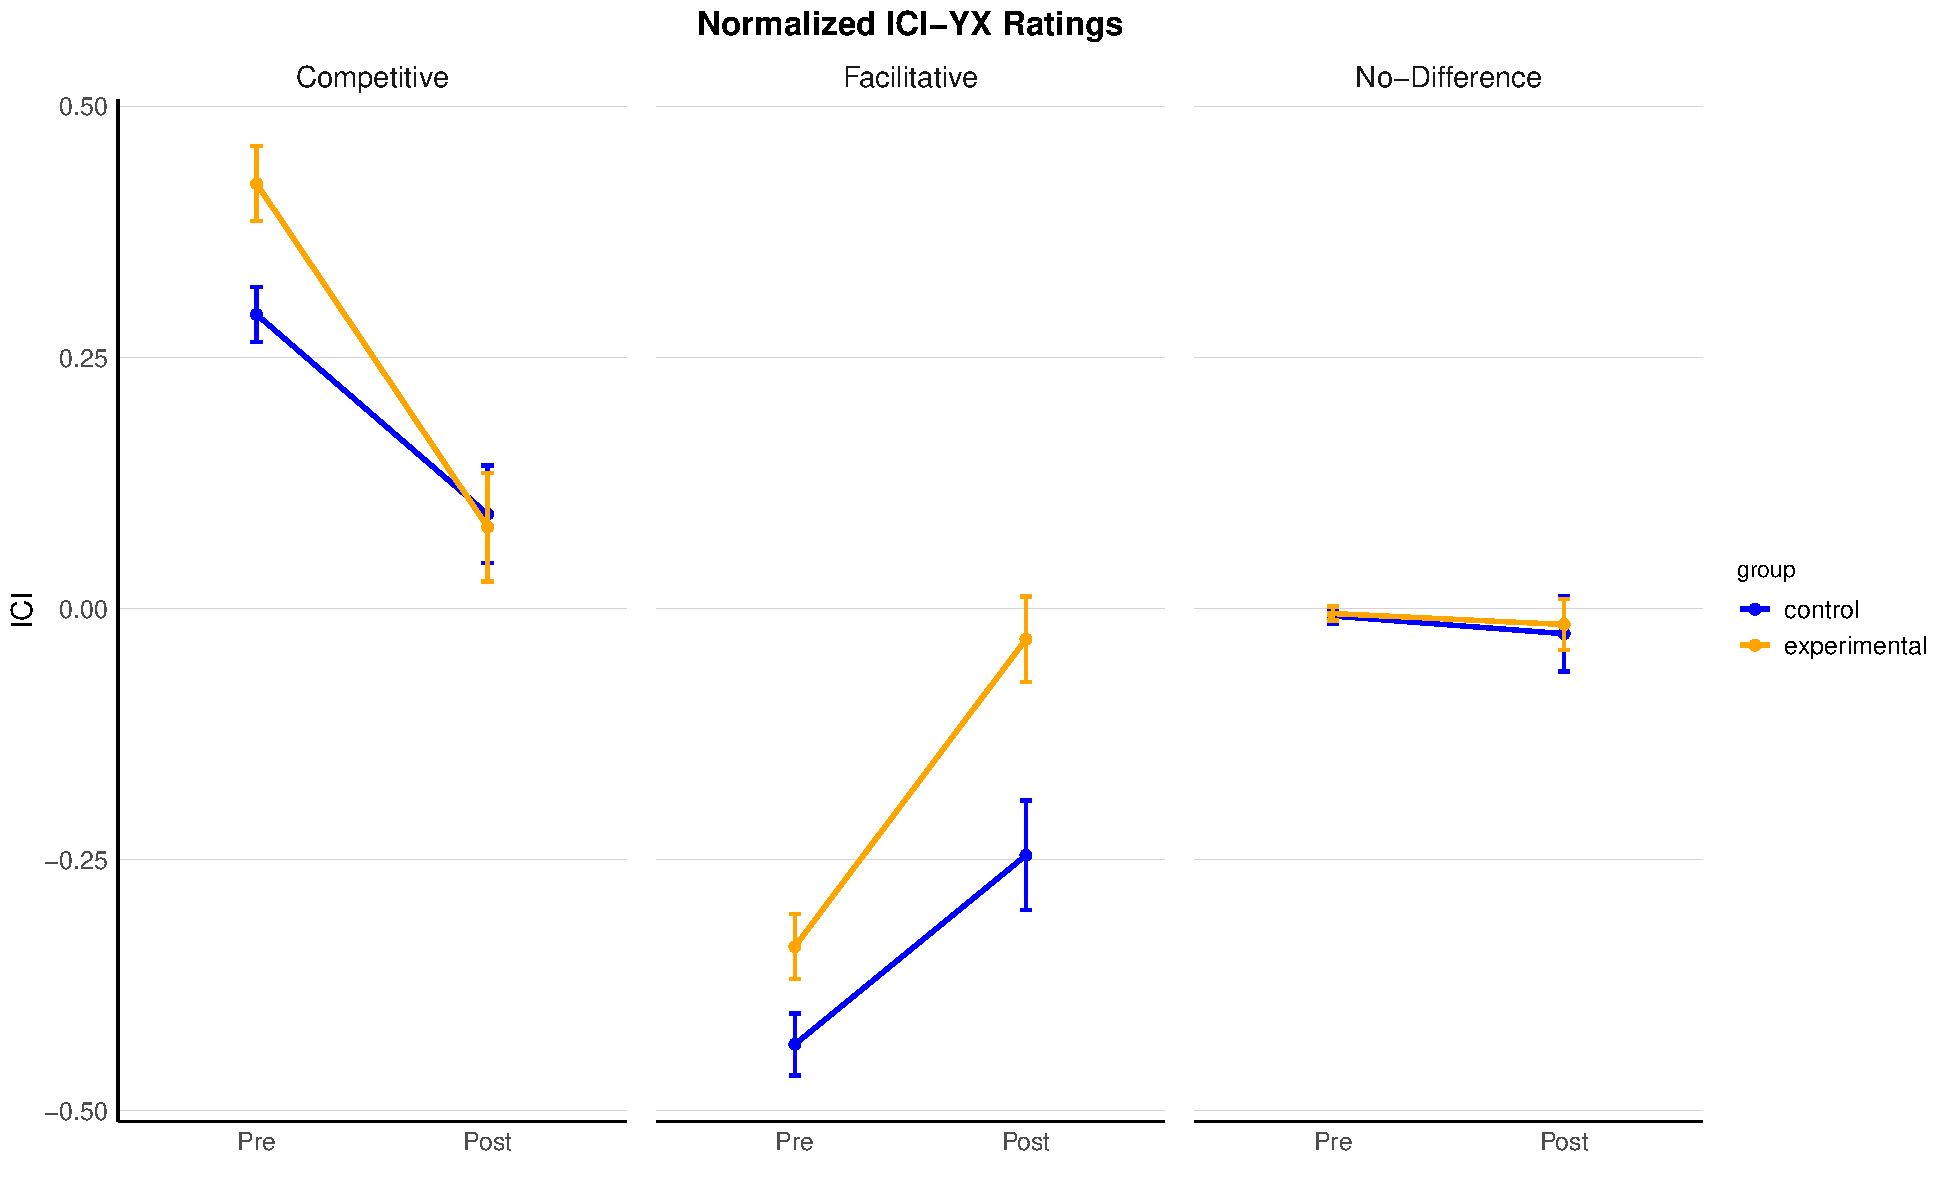
\includegraphics{index_files/figure-pdf/unnamed-chunk-44-1.pdf}

\begin{Shaded}
\begin{Highlighting}[]
\FunctionTok{plot\_ICI}\NormalTok{(df\_prp\_both, }\StringTok{\textquotesingle{}ICI\_YX\_dist\_pre\_norm\textquotesingle{}}\NormalTok{, }\StringTok{\textquotesingle{}ICI\_YX\_dist\_post\_norm\textquotesingle{}}\NormalTok{, }\StringTok{\textquotesingle{}style\_distance\textquotesingle{}}\NormalTok{, }\StringTok{\textquotesingle{}Normalized ICI{-}YX Distances\textquotesingle{}}\NormalTok{)}
\end{Highlighting}
\end{Shaded}

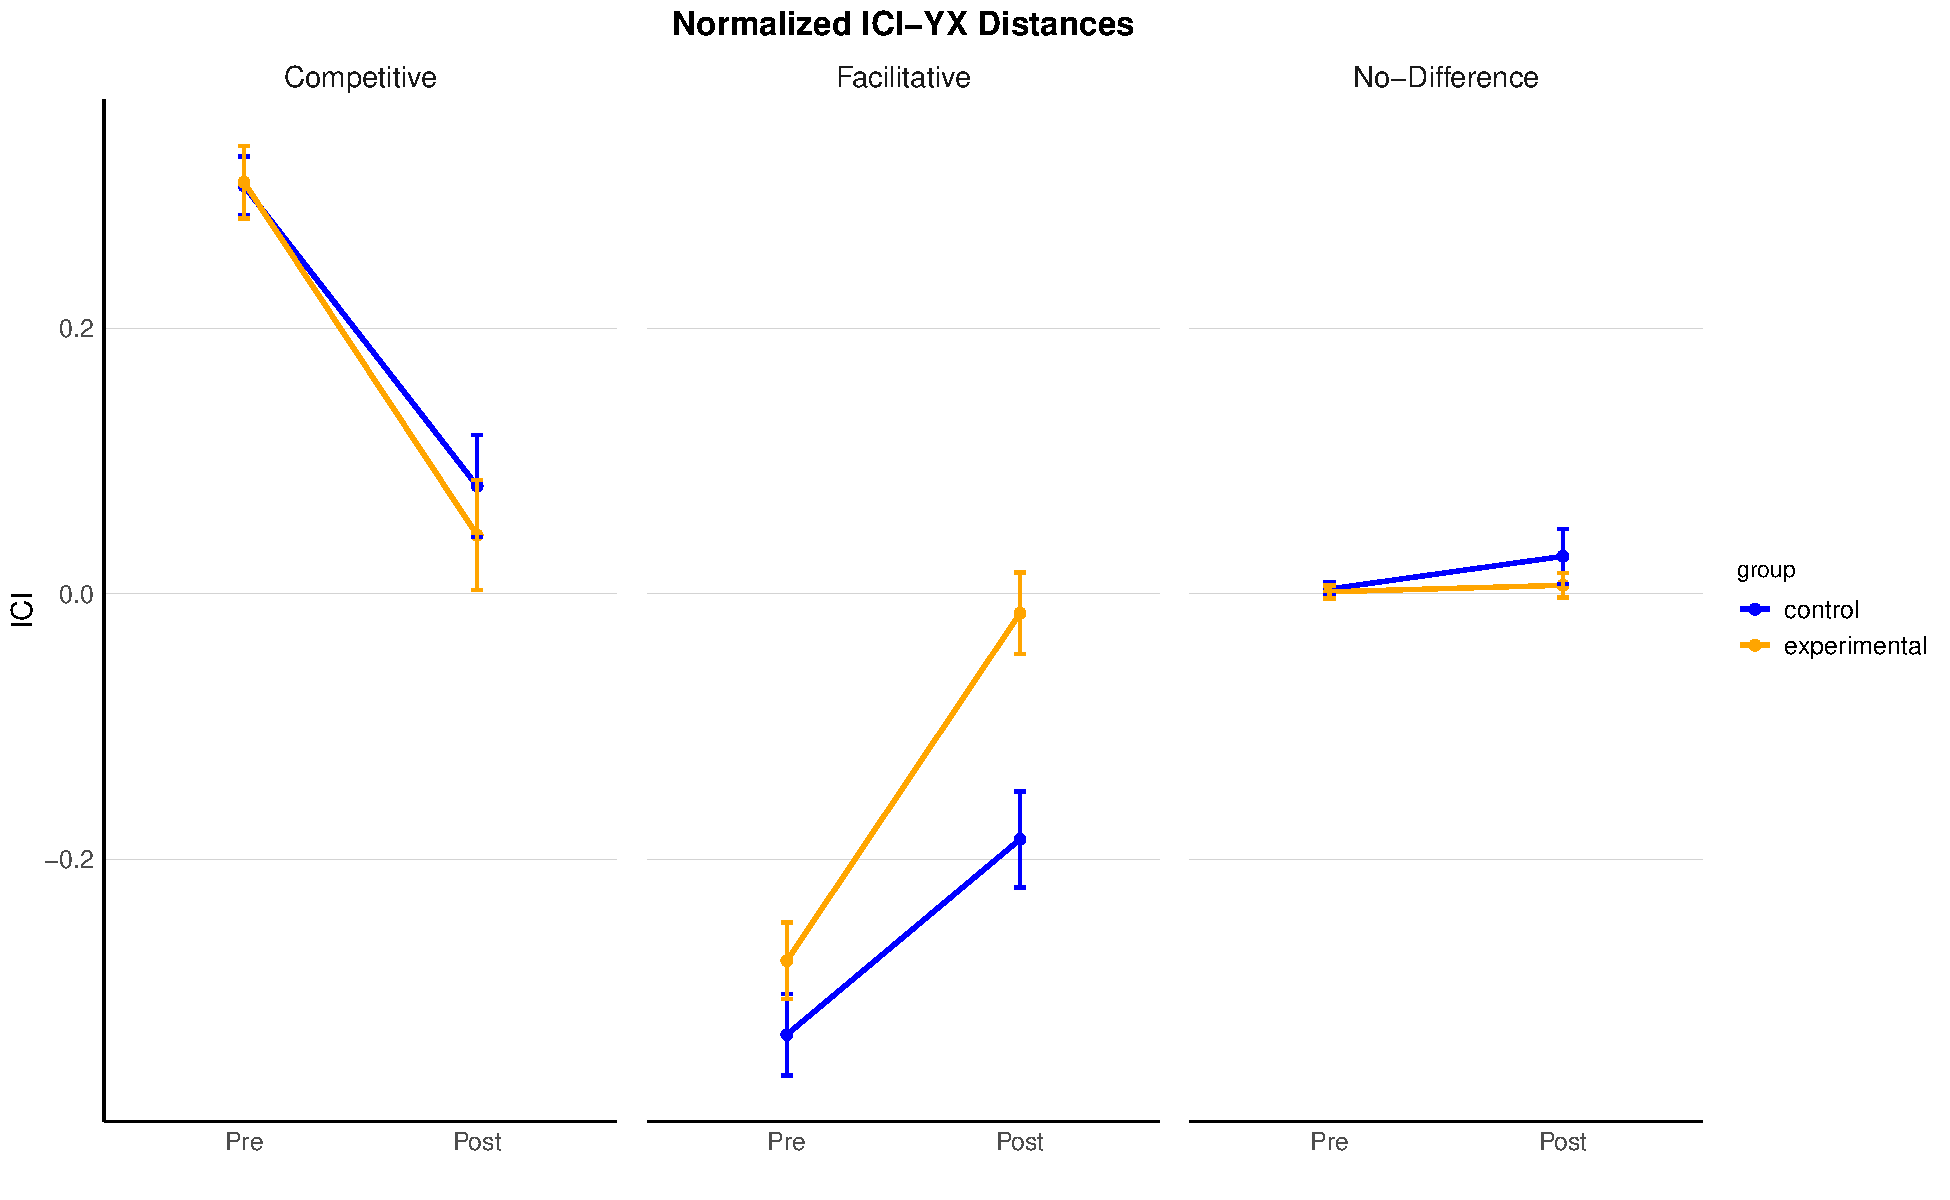
\includegraphics{index_files/figure-pdf/unnamed-chunk-44-2.pdf}

\subsection{Convert data to a long
format}\label{convert-data-to-a-long-format}

\begin{Shaded}
\begin{Highlighting}[]
\NormalTok{df\_prp\_long }\OtherTok{\textless{}{-}}\NormalTok{ df\_prp\_both }\SpecialCharTok{\%\textgreater{}\%}
  \FunctionTok{select}\NormalTok{(subjectID, group, style\_rating, style\_distance, ICI\_YX\_rating\_pre\_norm, ICI\_YX\_rating\_post\_norm, ICI\_YX\_dist\_pre\_norm, ICI\_YX\_dist\_post\_norm) }\SpecialCharTok{\%\textgreater{}\%}
  \FunctionTok{pivot\_longer}\NormalTok{(}\AttributeTok{cols =} \FunctionTok{c}\NormalTok{(ICI\_YX\_rating\_pre\_norm, ICI\_YX\_rating\_post\_norm, ICI\_YX\_dist\_pre\_norm, ICI\_YX\_dist\_post\_norm), }\AttributeTok{names\_to =} \StringTok{"Index"}\NormalTok{, }\AttributeTok{values\_to =} \StringTok{"value"}\NormalTok{) }
\CommentTok{\# save to CSV}
\FunctionTok{write\_csv}\NormalTok{(df\_prp\_long, }\StringTok{"./exp4{-}ICI.csv"}\NormalTok{)}
\end{Highlighting}
\end{Shaded}

\section{Result}\label{result}

\begin{enumerate}
\def\labelenumi{\arabic{enumi}.}
\tightlist
\item
  Stimulus types on normalized pre-manipulation rating indexes
\end{enumerate}

A one-way between-subjects ANOVA was conducted to examine the effect of
stimulus type (shape vs.~sound) on normalized pre-manipulation rating
indexes. The analysis revealed that the effect of stimulus type was not
statistically significant, F(1, 313) = 0.36, p = .55, η² = .001.

\begin{enumerate}
\def\labelenumi{\arabic{enumi}.}
\setcounter{enumi}{1}
\tightlist
\item
  Stimulus types on normalized pre-manipulation distance indexes
\end{enumerate}

A one-way between-subjects ANOVA was conducted to examine the effect of
stimulus type (shape vs.~sound) on normalized pre-manipulation distance
indexes. The analysis revealed that the effect of stimulus type was not
statistically significant, F(1, 313) = 1.008, p = .36, η² = .003.

\begin{enumerate}
\def\labelenumi{\arabic{enumi}.}
\setcounter{enumi}{2}
\tightlist
\item
  Correlations of anxiety, stress, and depression with rating
\end{enumerate}

Anxiety was not significantly correlated with participants'
pre-manipulation ratings, r(315) = -0.08, p = .18. Stress was not
significantly correlated with pre-manipulation ratings, r = -0.07, p =
.19. Depression was not significantly correlated with pre-manipulation
ratings, r = -0.06, p = .29.

\begin{enumerate}
\def\labelenumi{\arabic{enumi}.}
\setcounter{enumi}{3}
\tightlist
\item
  Correlations of anxiety, stress, and depression with Distance
\end{enumerate}

Anxiety was marginally negatively correlated with distance to the
object, r = -0.10, p = .07. Stress was significantly negatively
correlated with distance, r = -0.11, p = .04. Depression was not
significantly correlated with distance, r = -0.09, p = .11.

\begin{enumerate}
\def\labelenumi{\arabic{enumi}.}
\setcounter{enumi}{4}
\tightlist
\item
  Rating style and normalized pre-manipulation rating indexes
\end{enumerate}

A one-way between-subjects ANOVA was conducted to examine the effect of
rating style (Competitive, Facilitative, No-Difference) on participants'
normalized pre-manipulation ratings index. The results revealed a
statistically significant effect of rating style on normalized rating
indexes, F(2, 312) = 376.00, p \textless{} .001. The effect size was
large, η² = .71, 95\% CI {[}.67, 1.00{]}, indicating that approximately
71\% of the variance in normalized pre-manipulation rating indexes can
be attributed to rating style.

\begin{enumerate}
\def\labelenumi{\arabic{enumi}.}
\setcounter{enumi}{5}
\tightlist
\item
  Distance style on normalized pre-manipulation distance indexes
\end{enumerate}

A one-way between-subjects ANOVA was conducted to examine the effect of
distance style (Competitive, Facilitative, No-Difference) on
participants' normalized pre-manipulation distance index. The results
revealed a statistically significant effect of distance style on
distance indexes, F(2, 312) = 359.3, p \textless{} .001. The effect size
was large, η² = .70, 95\% CI {[}.66, 1.00{]}, indicating that
approximately 71\% of the variance in normalized pre-manipulation
distance index can be attributed to distance style.

\begin{enumerate}
\def\labelenumi{\arabic{enumi}.}
\setcounter{enumi}{6}
\tightlist
\item
  Rating style and group on normalized rating indexes
\end{enumerate}

A two-way mixed design ANOVA was conducted to examine the effects of
rating style (Competitive, Facilitative, No-Difference) and group
(Control, Experimental) on the change in normalized rating indexes from
pre- to post-manipulation. There was a significant main effect of rating
style, F(2, 309) = 49.28, p \textless{} .001, η² = .24, indicating that
the amount of change differed significantly across rating styles. There
was no significant main effect of group, F(1, 309) = 0.03, p = .859,
suggesting that, overall, control and experimental groups did not differ
in change scores. However, there was a significant interaction between
rating styles and group, F(2, 309) = 3.30, p = .038, indicating that the
effect of group on rating index change varied depending on the rating
style.

\begin{enumerate}
\def\labelenumi{\arabic{enumi}.}
\setcounter{enumi}{7}
\tightlist
\item
  Distance style and group on change in normalized distance indexes
\end{enumerate}

A two-way between-subjects ANOVA was conducted to examine the effects of
distance style (Competitive, Facilitative, No-Difference) and group
(Control, Experimental) on the change in participants' normalized
distance index from pre- to post-manipulation. There was a significant
main effect of distance style, F(2, 309) = 72.95, p \textless{} .001, η²
= .32, indicating that average distance index significantly differed
across styles. There was no significant main effect of group, F(1, 309)
= 0.38, p = .538, suggesting that control and experimental groups did
not differ overall in distance index. The interaction between distance
style and group was marginally significant, F(2, 309) = 2.52, p = .082,
η² ≈ .01, indicating a potential trend that the effect of group may
differ depending on distance style, though this did not reach
conventional levels of statistical significance.

\section{Discussion}\label{discussion}

\section{References}\label{references}




\end{document}
